% Формат А4, 12pt (ГОСТ Р 7.0.11-2011, 5.3.6)
\documentclass[a4paper,14pt]{extreport}

\input{packages}        % Подключаемые пакеты
\input{styles}          % Пользовательские стили
%%% Основные сведения %%%
\newcommand{\thesisAuthor}             % Диссертация, ФИО автора
{Григорьев Семён Вячеславович}
\newcommand{\thesisTitle}              % Диссертация, название
{Cинтаксический анализ динамически формируемых строковых выражений}
\newcommand{\thesisSpecialtyNumber}    % Диссертация, специальность, номер
{05.13.11}
\newcommand{\thesisSpecialtyTitle}     % Диссертация, специальность, название
{Математическое и программное обеспечение вычислительных машин, комплексов и компьютерных сетей}
\newcommand{\thesisDegree}             % Диссертация, научная степень
{кандидата физико-математических наук}
\newcommand{\thesisCity}               % Диссертация, город защиты
{Санкт-Петербург}
\newcommand{\thesisYear}               % Диссертация, год защиты
{2015}
\newcommand{\thesisOrganization}       % Диссертация, организация
{кафедре системного программирования математико-механического факультета Санкт-Петербургского государственного университета}

\newcommand{\supervisorFio}            % Научный руководитель, ФИО
{Кознов Дмитрий Владимирович}
\newcommand{\supervisorRegalia}        % Научный руководитель, регалии
{кандидат физико-математических наук, доцент}

\newcommand{\opponentOneFio}           % Оппонент 1, ФИО
{Ицыксон Владимир Михайлович}
\newcommand{\opponentOneRegalia}       % Оппонент 1, регалии
{кандидат технических наук, доцент}
\newcommand{\opponentOneJobPlace}      % Оппонент 1, место работы
{ФГБОУ ВПО ``Санкт-Петербургский государственный политехнический университет''}
\newcommand{\opponentOneJobPost}       % Оппонент 1, должность
{\todo{}}

\newcommand{\opponentTwoFio}           % Оппонент 2, ФИО
{\todo{ }}
\newcommand{\opponentTwoRegalia}       % Оппонент 2, регалии
{\todo{ }}
\newcommand{\opponentTwoJobPlace}      % Оппонент 2, место работы
{\todo{ }}
\newcommand{\opponentTwoJobPost}       % Оппонент 2, должность
{\todo{ }}

\newcommand{\leadingOrganizationLines} % Ведущая организация, дополнительные строки
{\\~\\~\\~}
\newcommand{\leadingOrganizationTitle} % Ведущая организация, дополнительные строки
{\todo{ }}

\newcommand{\defenseDate}              % Защита, дата
{\todo{}}% г.~в~  часов}}
\newcommand{\defenseCouncilNumber}     % Защита, номер диссертационного совета
{Д 212.232.51}
\newcommand{\defenseCouncilTitle}      % Защита, учреждение диссертационного совета
{Санкт-Петербургского государcтвенного университета}
\newcommand{\defenseCouncilAddress}    % Защита, адрес учреждение диссертационного совета
{198504, Санкт-Петербург, Петродворец, Университетский пр., 28, математико-механический факультет, ауд. 405}

\newcommand{\defenseSecretaryFio}      % Секретарь диссертационного совета, ФИО
{Косовский Николай Кириллович}
\newcommand{\defenseSecretaryRegalia}  % Секретарь диссертационного совета, регалии
{д.ф.-м.н., профессор}

\newcommand{\synopsisLibrary}          % Автореферат, название библиотеки
{\todo{ }}
\newcommand{\synopsisDate}             % Автореферат, дата рассылки
{\todo{  }}%года}}
            % Основные сведения

\newtheoremstyle{mystyle}%                % Name
  {}%                                     % Space above
  {}%                                     % Space below
  {\itshape}%                             % Body font
  {}%                                     % Indent amount
  {\scshape}%                            % Theorem head font
  {.}%                                    % Punctuation after theorem head
  { }%                                    % Space after theorem head, ' ', or \newline
  {}%                                     % Theorem head spec (can be left empty, meaning `normal')

\theoremstyle{mystyle}

%\usepackage{etoolbox}
%\makeatletter
%\patchcmd{\@thm}{\thm@headfont{\scshape}}{\thm@headfont{\scshape\bfseries}}{}{}
%\patchcmd{\@thm}{\thm@notefont{\fontseries\mddefault\upshape}}{}{}{}
%\makeatother

\begin{document}

\algtext*{EndWhile}% Remove "end while" text
\algtext*{EndIf}% Remove "end if" text
\algtext*{EndFor}% Remove "end for" text
\algtext*{EndFunction}% Remove "end function" text
%\declaretheoremstyle[headfont=\normalfont]{normalhead}
%\declaretheorem[style=normalhead]{example}
%\theoremheaderfont{\textsc}
\newtheorem{mydef}{Определение}
\renewcommand{\lstlistingname}{Листинг}
\renewcommand\listingscaption{Листинг}


\input{names}           % Переопределение именований

% Структура диссертации (ГОСТ Р 7.0.11-2011, 4)
%% Если что-то забыли, при компиляции будут ошибки Undefined control sequence \my@title@<что забыли>@ru
%% Если англоязычная титульная страница не нужна, то ее можно просто удалить.
\filltitle{ru}{
    %% Актуально только для курсовых/практик. ВКР защищаются не на кафедре а в ГЭК по направлению, 
    %%   и к моменту защиты вы будете уже не в группе.
    chair              = {Кафедра системного программирования},
    group              = {17Б.11-мм},
    %% Макрос filltitle ненавидит пустые строки, поэтому обязателен хотя бы символ комментария на строке
    %% Актуально всем.
    title              = {Реализация алгоритма поиска путей в графовых базах данных через тензорное произведение на GPGPU},
    % 
    %% Здесь указывается тип работы. Возможные значения:
    %%   coursework - отчёт по курсовой работе;
    %%   practice - отчёт по учебной практике;
    %%   prediploma - отчёт по преддипломной практике;
    %%   master - ВКР магистра;
    %%   bachelor - ВКР бакалавра.
    type               = {bachelor},
    author             = {Орачев Егор Станиславович},
    % 
    %% Актуально только для ВКР. Указывается код и название направления подготовки. Типичные примеры:
    %%   02.03.03 <<Математическое обеспечение и администрирование информационных систем>>
    %%   02.04.03 <<Математическое обеспечение и администрирование информационных систем>>
    %%   09.03.04 <<Программная инженерия>>
    %%   09.04.04 <<Программная инженерия>>
    %% Те, что с 03 в середине --- бакалавриат, с 04 --- магистратура.
    specialty          = {09.03.04 <<Программная инженерия>>},
    % 
    %% Актуально только для ВКР. Указывается шифр и название образовательной программы. Типичные примеры:
    %%   СВ.5006.2017 <<Математическое обеспечение и администрирование информационных систем>>
    %%   СВ.5162.2020 <<Технологии программирования>>
    %%   СВ.5080.2017 <<Программная инженерия>>
    %%   ВМ.5665.2019 <<Математическое обеспечение и администрирование информационных систем>>
    %%   ВМ.5666.2019 <<Программная инженерия>>
    %% Шифр и название программы можно посмотреть в учебном плане, по которому вы учитесь. 
    %% СВ.* --- бакалавриат, ВМ.* --- магистратура. В конце --- год поступления (не обязательно ваш, если вы были в академе/вылетали).
    programme          = {СВ.5080.2017 <<Программная инженерия>>},
    % 
    %% Актуально только для ВКР, только для матобеса и только 2017-2018 годов поступления. Указывается профиль подготовки, на котором вы учитесь.
    %% Названия профилей можно найти в учебном плане в списке дисциплин по выбору. На каком именно вы, вам должны были сказать после второго курса (можно уточнить в студотделе).
    %% Вот возможные вариканты:
    %%   Математические основы информатики
    %%   Информационные системы и базы данных
    %%   Параллельное программирование
    %%   Системное программирование
    %%   Технология программирования
    %%   Администрирование информационных систем
    %%   Реинжиниринг программного обеспечения
    % profile            = {Системное программирование},
    % 
    %% Актуально всем.
    supervisorPosition = {Доцент кафедры информатики, к.\,ф.-м.\,н.},
    supervisor         = {С. В. Григорьев},
    % 
    %% Актуально только для практик и курсовых. Если консультанта нет, закомментировать или удалить вовсе.
    % consultantPosition = {должность ООО <<Место работы>> степень},
    % consultant         = {К.К. Консультант},
    %
    %% Актуально только для ВКР.
    reviewerPosition   = {Разработчик биоинформатического ПО, ЗАО “БИОКАД”},
    reviewer           = {А.С. Хорошев},
}

\filltitle{en}{
    chair              = {Software Engineering},
    group              = {17B.11-mm},
    title              = {Context-Free path querying by tensor product for graph databases on GPGPU},
    type               = {bachelor},
    author             = {Egor Orachev},
    % 
    %% Possible choices:
    %%   02.03.03 <<Software and Administration of Information Systems>>
    %%   02.04.03 <<Software and Administration of Information Systems>>
    %%   09.03.04 <<Software Engineering>>
    %%   09.04.04 <<Software Engineering>>
    %% Те, что с 03 в середине --- бакалавриат, с 04 --- магистратура.
    specialty          = {09.03.04 <<Software Engineering>>},
    % 
    %% Possible choices:
    %%   СВ.5006.2017 <<Software and Administration of Information Systems>>
    %%   СВ.5162.2020 <<Programming Technologies>>
    %%   СВ.5080.2017 <<Software Engineering>>
    %%   ВМ.5665.2019 <<Software and Administration of Information Systems>>
    %%   ВМ.5666.2019 <<Software Engineering>>
    programme          = {СВ.5080.2017 <<Software Engineering>>},
    % 
    %% Possible choices:
    %%   Mathematical Foundations of Informatics
    %%   Information Systems and Databases
    %%   Parallel Programming
    %%   System Programming
    %%   Programming Technology
    %%   Information Systems Administration
    %%   Software Reengineering
    % profile            = {Software Engineering},
    % 
    %% Note that common title translations are:
    %%   кандидат наук --- C.Sc. (NOT Ph.D.)
    %%   доктор ... наук --- Sc.D.
    %%   доцент --- docent (NOT assistant/associate prof.)
    %%   профессор --- prof.
    supervisorPosition = {C.Sc., docent},
    supervisor         = {S.V. Grigorev},
    % 
    % consultantPosition = {position at ``Company'', degree if present},
    % consultant         = {C.C. Consultant},
    % %
    reviewerPosition   = {Bioinformatics Software Engineer, BIOCAD},
    reviewer           = {A.S. Khoroshev},
}           % Титульный лист
\input{contents}        % Оглавление
\section{Introduction}

Scalable high-performance graph analysis is an actual challenge.
There is a big number of ways to attack this challenge~\cite{Coimbra2021} and the first promising idea is to utilize general-purpose graphic processing units (GPGPU).
Such existing solutions, as CuSha~\cite{10.1145/2600212.2600227} and Gunrock~\cite{7967137} show that utilization of GPUs can improve the performance of graph analysis, moreover it is shown that solutions may be scaled to multi-GPU systems.
But low flexibility and high complexity of API are problems of these solutions.

The second promising thing which provides a user-friendly API for high-performance graph analysis algorithms creation is a GraphBLAS API~\cite{7761646} which provides linear algebra based building blocks to create graph analysis algorithms.
The idea of GraphBLAS is based on a well-known fact that linear algebra operations can be efficiently implemented on parallel hardware.
Along with that, a graph can be natively represented using matrices: adjacency matrix, incidence matrix, etc.
While reference CPU-based implementation of GraphBLAS, SuiteSparse:GraphBLAS~\cite{10.1145/3322125}, demonstrates good performance in real-world tasks, GPU-based implementation is challenging.

One of the challenges in this way is that real data are often sparse, thus underlying matrices and vectors are also sparse, and, as a result, classical dense data structures and respective algorithms are inefficient. 
So, it is necessary to use advanced data structures and procedures to implement sparse linear algebra, but the efficient implementation of them on GPU is hard due to the irregularity of workload and data access patterns.
Though such well-known libraries as cuSPARSE show that sparse linear algebra operations can be efficiently implemented for GPGPU, it is not so trivial to implement GraphBLAS on GPGPU. 
First of all, it requires \textit{generic} sparse linear algebra, thus it is impossible just to reuse existing libraries which are almost all specified for operations over floats.
The second problem is specific optimizations, such as masking fusion, which can not be natively implemented on top of existing kernels.
Nevertheless, there is a number of implementations of GraphBLAS on GPGPU, such as GraphBLAST~\cite{yang2019graphblast}, GBTL~\cite{7529957}, which show that GPGPUs utilization can improve the performance of GraphBLAS-based graph analysis solutions.
But these solutions are not portable because they are based on Nvidia Cuda stack.
Moreover, the scalability problem is not solved: all these solutions support only single-GPU, not multi-GPU computations.

To provide portable GPU implementation of GraphBLAS API we developed a \textit{SPLA} library\footnote{Source code available at: \url{https://github.com/JetBrains-Research/spla}}.
This library utilizes OpenCL for GPGPU computing to be portable across devices of different vendors.
Moreover, it is initially designed to utilize multiple GPGPUs to be scalable.
To sum up, the contribution of this work is the following.
\begin{itemize}
    \item Design of portable GPU GraphBLAS implementation proposed. The design involves the utilization of multiple GPUS. Additionally, the proposed design is aimed to simplify library tuning and wrappers for different high-level platforms and languages creation. 
    \item Subset of GraphBLAS API, including such operations as masking, matrix-matrix multiplication, matrix-matrix e-wise addition, is implemented. The current implementation is limited by COO and CSR matrix representation format and uses basic algorithms for some operations, but work in progress and more data formats will be supported and advanced algorithms will be implemented in the future.
    \item Preliminary evaluation on such algorithms as breadth-first search (BFS) and triangles counting (TC), and real-world graphs shows portability across different vendors and promising performance: for some problems Spla is comparable with GraphBLAST. Surprisingly, for some problems, the proposed solution on embedded Intel graphic card shows better performance than SuiteSparse:GraphBLAS on the respective CPU. At the same time, the evaluation shows that further optimization is required.
\end{itemize}     % Введение
\section{Обзор}

Для того чтобы упростить ход рассуждений, касающихся контекстно-свободных грамматик, в данной работе используется понятие \textit{рекурсивного автомата} --- абстракции, позволяющей задавать произвольную КС-грамматику.
Ее описание приводится в первом параграфе обзора. 
Второй параграф посвящен вопросу о разрешимости задачи синтаксического анализа контекстно-свободного представления данных и его связи с фундаментальными проблемами теории формальных языков.

Предлагаемый в данной работе алгоритм основан на алгоритме синтаксического анализа регулярных множеств, который, в свою очередь, явлется модификацией алгоритма обобщенного синтаксического анализа Generalized LL. 
Об этих алгоритмах, а также о проекте, в рамках которого проведена разработка предложенного решения, также будет рассказано в обзоре.

\subsection{Рекурсивные автоматы и КС-грамматики}
Введем понятие рекурсивного автомата, которое потребуется для дальнейшего изложения

\begin{defn}
	Рекурсивный автомат R --- это пятерка $(\Sigma, Q, \delta, q_0, q_f)$, где $\Sigma$ --- конечное множество терминальных символов, $Q$ --- конечное множество состояний автомата, $\delta : Q \times (\Sigma \cup Q) \rightarrow 2^Q$ --- функция переходов, $q_0 \in Q$ --- начальное состояние, $q_f$ --- конечное состояние. 
\end{defn}

Можно заметить, что данное определение практически идентично определению стандартного конечного автомата. 
Единственное отличие состоит в том, что метками на ребрах рекурсивного автомата могут как терминальные символы (терминальные переходы), так и состояния (нетерминальные переходы).
Класс рекурсивных автоматов обладает такой же выразительностью, как и контекстно-свободные грамматики, т.е. позволяет описать любой контекстно-свободный язык. 
Более того, грамматика тривиальным образом может быть преобразована в рекурсивный автомат (обратное тоже верно) \cite{tellier2006ra}. 
Пример рекурсивного автомата, построенного по грамматике, можно увидеть на рисунке \ref{fig:ra_ex}.

\begin{figure}[h]
	\centering
	\begin{subfigure}[b]{0.45\textwidth}
		\centering
		$$
		\begin{array}{crcl}
		&S' & ::= & S \\
		&S  & ::= & \texttt{[ } S \texttt{ ]}\\
		&S  & ::= & \mbox{\texttt{a}}
		\end{array}
		$$
		\caption{Грамматика $G_1$}
	\end{subfigure}
	~
	\begin{subfigure}[b]{0.45\textwidth}
		\centering
		\includegraphics[width=4cm]{pictures/ra_example.pdf}
		\caption{Рекурсивный автомат для $G_1$}
	\end{subfigure}
	\caption{Преобразование между грамматикой и рекурсивным автоматом}
	\label{fig:ra_ex}
\end{figure}


\subsection{Разрешимость задачи синтаксического анализа контекстно-свободного представления}
Как было сказано ранее, задачу поиска шаблона, при условии, что и шаблон, и данные, в которых осуществляется поиск, представлены контекстно-свободными грамматиками, мы назовем синтаксическим анализом контекстно-свободного представления. 

Для доказательства предложений, сформулированных далее, будет использоваться следующая теорема \cite{Nederhof}.

\begin{theorem}[Nederhof, Satta]
	Пусть $G_1$ --- произвольная контекстно-свободная грамматика, $G_2$ --- грамматика, которая не содержит непосредственной или скрытой рекурсий. Тогда проблема проверки пустоты пересечения языков, порождаемых данными грамматиками, относится к классу PSPACE-complete.
\end{theorem}

Рассмотрим случай, когда грамматика данных задает ровно одну строку. Пусть $G_t$ --- произвольная КС-грамматика, задающая шаблоны для поиска, а $G_d$ --- КС-грамматика, которая не содержит непосредственной или скрытой рекурсий. $L(G_t)$ и $L(G_d)$ --- языки, порождаемые грамматиками, при этом $L(G_d) = \{\omega\}$, где $\omega$ --- исходные данные, к которым был применен алгоритм сжатия. 
Необходимо определить, существуют ли такие строки $\omega'$, что $\omega' \in L(G_t)$ и $\omega'$ --- подстрока $\omega$.

%т.е. $\omega' \in L_{sub}(\omega)$, где $L_{sub}(s)$ --- обозначение для языка, состоящего из всех подстрок заданной строки $s$. Отметим, что $L_{sub}$ относится к классу регулярных языков, так как множество всех подстрок конечно. 

\begin{prop}
	При выполнении описанных условий задача синтаксического анализа КС-представления разрешима.
\end{prop}

\begin{proof}
Пользуясь эквивалентностью представлений, можно записать грамматику $G_d$ в виде рекурсивного автомата $R_d$. Рассмотрим рекурсивный автомат $R_{i,\,j}$, полученный из $R_d$ путем замены стартового состояния на $i \in Q(R_d)$ и назначения терминирующего (финального, из которого не может быть совершено переходов) состояния $j \in Q(R_d)$. Такой автомат описывает грамматику, которая является представленим некоторой подстроки $\omega$. 
%В таком случае, рекурсивный автомат $R_{i,\,j}$, полученный из $R_d$ путем замены стартового и конечного состояний на $i, j \in Q(R_d)$ соответственно, описывает грамматику, которая является представленим некоторой подстроки $\omega$. 
Рассмотрев все возможные пары $i$ и $j$, получаем конечное множество грамматик, для каждой из которых необходимо проверить, содержится ли строка, порождаемая ей, в языке $L(G_t)$. 
Согласно теореме 1, такая проверка является разрешимой задачей и принадлежит к классу PSPACE-complete.
\end{proof}

Отдельно отметим, что для описанных процедур используется лишь исходный автомат, эквивалентный грамматике $G_d$. 
Условия задачи поиска шаблонов непосредственно в контекстно-свободном представлении, таким образом, выполняются. 
Верна также разрешимость более общей задачи.

\begin{prop}
	Пусть грамматика $G_d$ задает конечное множество строк $L(G_d) = \{\omega_1, \, \dots \, , \omega_n \}$. Необходимо определить, существуют ли строки $\omega'$, для которых верно: $\omega' \in L(G_t)$ и $\omega'$ --- подстрока одной из строк $\omega_i \in L(G_d)$. Данная задача разрешима и принадлежит классу PSPACE-complete.
\end{prop}

\begin{proof}
	Как и в предыдущем доказательстве, используем запись грамматики в виде рекурсивного автомата $R_d$ и рассмотрим автоматы $R_{i, j}$. В данном случае каждый из этих автоматов представляет собой грамматику, которая порождает некоторое конечное множество подстрок исходных строк из $L(G_d)$. Проверка пустоты пересечения такой грамматики с $G_t$ также соответствует условиям теоремы 1.
\end{proof}

В случае, когда грамматика $G_d$ представляет собой бесконечный регулярный язык (т.е. содержит левую и/или правую рекурсию), разрешимость задачи поиска шаблонов установить не удается. Подход, использованный ранее в доказательстве предложений, не может быть применен, так как части рекурсивного автомата, представляющего грамматику $G_d$, также могут содержать рекурсивные переходы, что выходит за рамки условия теоремы 1. Проверка разрешимости и определение класса сложности задачи проверки пустоты пересечения произвольной и регулярной КС-грамматик в настоящее время остаются открытыми проблемами \cite{Nederhof}.

%Пусть $G$ --- произвольная КС-грамматика, $M$ --- конечный автомат. Тогда задача проверки
%\begin{itemize}
%	\item включения языков ($L(M) \subseteq L(G)$) --- неразрешима
%	\item пустоты пересечения ($L(M) \cap L(G) = \emptyset$) --- разрешима (т.к. в пересечении не более чем КС-язык) за полиномиальное время \cite{Hunt}
%	\item регулярности языка $L(G)$ --- неразрешима \cite{Greibach1968}
%\end{itemize} 
%
%Если использовать представление регулярного языка $L(M)$ в виде КС-грамматики $G_r$, то задача проверки пустоты пересечения ($L(G_r) \, \cap \, L(G) = \emptyset$) становится немного интереснее: если $G_r$ 
%\begin{itemize}
%	\item нерекурсивная --- задача из PSPACE \cite{Nederhof} (точнее результата нет (я не нашел, по крайней мере))
%	\item лево- или праволинейная --- ничего не известно (см. последний абзац заключения из \cite{Nederhof})
%	\item принадлежит еще более широкому классу --- тем более ничего не известно
%\end{itemize}

%Еще немного про вложенную рекурсию и регулярность языка. Грамматика без вложенной рекурсии (NSE) порождает регулярный язык \cite{Chomsky} (обратное тоже верно, для регулярного языка можно построить NSE грамматику, т.к. праволинейная, например, --- частный случай NSE). Существует алгоритм, который позволяет проверять грамматику на наличие вложенной рекурсии за полином \cite{Anselmo}. Однако, грамматика с вложенной рекурсией тоже может порождать регулярный язык \cite{Andrei2004}, поэтому задача о проверке регулярности языка, порождаемого КС-грамматикой, остается неразрешимой. 

\subsection{GLL-алгоритм и его модификации}

Классические алгоритмы нисходящего и восходящего синтаксического анализа предполагают использование грамматики, которая является в достаточной мере однозначной. 
В противном случае, управляющие таблицы анализаторов содержат конфликты, из-за чего нельзя гарантировать корректное поведение на любых входных данных. 
Для работы с сильно неоднозначными грамматикам используются алгоритмы \textit{обобщенного синтаксического анализа}, которые позволяют рассмотреть все возможные пути разбора строки и построить соответствующие деревья вывода.
Поиск шаблонов не требует наличия деревьев вывода, поэтому в дальнейшем алгоритмы синтаксического анализа рассматриваются только как механизм, позволяющий определить принадлежность строки языку.

\subsubsection{Оригинальный GLL-алгоритм}

Generalized LL (GLL) \cite{gll} --- алгоритм, обобщающий идеи нисходящего синтаксического анализа. GLL, в отличие от стандартных LL-алгоритмов, позволяет использовать для анализа произвольную \linebreak контекстно-свободную грамматику, в том числе содержащую леворекурсивные правила. Вместе с тем, GLL наследует такие полезные свойства алгоритмов нисходящего анализа, как непосредственная связь с грамматикой и простота отладки и диагностики ошибок.

Для обработки неоднозначностей GLL разделяет стек анализатора на несколько ветвей, каждая из которых соответствует возможному пути разбора. При таком подходе необходимо компактное представление множества стеков, в качестве которого выступает Graph Structured Stack (GSS). В работе \cite{Afroozeh2015gss} была представлена модификация GSS, которая позволяет увеличить эффективность GLL-анализа. Вершины такого представления хранят в себе номер нетерминала и позицию в строке, с которой начался разбор подстроки, соответствующей ему. На ребрах хранятся позиции в грамматике (вида $X \rightarrow \alpha A \cdot \beta$), на которые необходимо вернуться после завершения разбора нетерминала. 
%При помощи GSS также решается проблема бесконечного роста стеков при обработке левой рекурсии: при попытке создать вершину, которая уже существует, в граф добавится

Основной идеей GLL является использование дескрипторов, позволяющих полностью описывать состояние анализатора в текущий момент времени.

\begin{defn}
	Дескриптор --- это тройка (L, u, i), где
	\begin{itemize}
		\setlength\itemsep{0em}
		\item L --- текущая позиция в грамматике вида $A \rightarrow \alpha \cdot \beta$
		\item u --- текущая вершина GSS
		\item i --- позиция во входном потоке 
	\end{itemize}
\end{defn}  

В процессе работы поддерживается глобальная очередь дескрипторов. В начале каждого шага исполнения алгоритм берет следующий в очереди дескриптор и производит действия в зависимости от позиции в грамматике и текущего входного символа, передвигая соответствующие указатели. 
При наличии конфликтов в грамматике алгоритм добавляет дескрипторы для каждого возможного пути анализа в конец очереди.

\subsubsection{Поддержка грамматик в EBNF}

В работе Артема Горохова \cite{Gorokhov2017ebnf} была описана модификация GLL, которая позволяет использовать грамматики, записанные в расширенной форме Бэкуса-Наура (EBNF). Грамматика такого вида трансформируется в соответствующий рекурсивный автомат, в котором затем минимизируется количество состояний. Синтаксический анализ производится без построения управляющих таблиц: алгоритм обходит рекурсивный автомат в соответствии со входным потоком символов. При обработке текущего дескриптора $(C_S, C_U, i)$, где $C_S$ --- вершина автомата (эквивалент позиции в грамматике), $C_U$ --- вершина GSS, $i$ --- позиция в строке, могут возникать следующие ситуации.

\begin{itemize}
	\item $C_S$ --- финальное состояние. Показывает, что разбор текущего нетерминала был завершен. Необходимо осуществить возврат из $C_U$ по меткам на исходящих из нее ребрах.
	\item Присутствует нетерминальный переход из $C_S$. В данном случае необходимо начать разбор указанного нетерминала $X$. Для этого в GSS должна быть создана новая вершина $(X, i)$, если она не создавалась ранее, а текущая вершина автомата изменена на стартовую для $X$.
	\item Присутствует терминальный переход из $C_S$. Необходимо сравнить терминал на ребре автомата с текущим входным символом. Если они совпадают, то осуществить переход в вершину автомата, на которую указывает ребро, и передвинуть указатель в строке.
\end{itemize}

За счет уменьшения количества состояния в автомате удается достичь прироста в производительности по сравнению со стандартным GLL-алгоритмом. 

\subsubsection{Синтаксический анализ графов}

Стандартными входными данными для алгоритмов синтаксического анализа являются линейные последовательности токенов. На основе GLL был разработан алгоритм, который позволяет производить синтаксический анализ регулярных множеств строк, представленных в виде конечного автомата (который, в свою очередь, является ориентированным графом с токенами на ребрах).

Поддержка нелинейного входа не потребовала существенных изменений в оригинальном алгоритме. Дескрипторы модифицированного алгоритма хранят номер вершины входного графа вместо позиции в строке. Также, на шаге исполнения просматривается не единственный текущий символ, а множество символов на ребрах, исходящих из текущей вершины.

Производительность данного алгоритма, как и обычного GLL, может быть увеличена при помощи представления входной грамматики в виде рекурсивного автомата. В таком случае, алгоритм будет производить обход двух автоматов --- рекурсивного и конечного. Ситуации, возникающие при обработке дексрипторов, не отличаются от описанных ранее ситуаций для линейного входа. Псевдокод данной модификации приведен в приложении.

\subsection{Проект YaccConstructor}

YaccConstructor --- исследовательский проект лаборатории языковых инструментов JetBrains на математико-механическом факультете СПбГУ, направленный на исследования в области лексического и синтаксического анализа. Проект включает в себя одноименную модульную платформу для разработки лексических и синтаксических анализаторов, содержащую большое количество компонент: язык описания грамматик YARD, преобразования над грамматиками и др. Основным языком разработки является F$\#$.

Ранее в рамках YaccConstructor были реализованы генераторы GLL-анализаторов, описание которых было приведено в данном обзоре. 

\chapter{Алгоритм синтаксического анализа регулярной аппроксимации} \label{AlgoDescr}

В данной главе формально описана задача синтаксического анализа динамически формируемых выражений, а так же изложен алгоритм её решения. Также сформулированы и доказаны утверждения о корректности данного алгоритма.

\section{Постановка задачи}

Анализируемая программа $\mathcal{P}$ является генератором выражений и таким образом задаёт некоторый язык $L_1$. Предположим, что $\mathcal{P}$ взаимодействует с базой данных с помощью динамически формируемых выражений. В этом случае мы говорим, что $\mathcal{P}$ использует динамический SQL, подразумевая, что программой генерируются выражения на языке SQL. Однако это не совсем корректно, так как программа может, например, содержать ошибку и некоторые из построенных ей выражений не будут корректными SQL-выражениями. Кроме того, программа $\mathcal{P}$ может генерировать не все возможные выражения на SQL. Таким образом, в этом случае $L_1\neq$~SQL.

С другой стороны, может быть задан эталонный язык $L_2$ --- язык, которому должны принадлежать все выражения генерируемые программой $\mathcal{P}$. Как правило $L_2$ описывается с помощью контекстно-свободной грамматики. Например, это может быть грамматика конкретного диалекта SQL, взятая из документации.

В результате мы имеем описание двух языков, и задача проверки корректности выражений, генерируемых $\mathcal{P}$, может быть сформулирована как проверка вложенности языка $L_1$ в язык $L_2$. Однако в рамках данной работы нас интересует не просто вложенность языков, а построение деревьев вывода. Как уже говорилось, язык $L_2$ может быть задан с помощью грамматики. Пусть задана грамматика $G$, такая, что $L_2 = L(G)$, тогда задача синтаксического анализа динамически формируемых выражений может быть поставлена следующим образом: для всех цепочек $\omega \in L_1$, выводимых в грамматике $G$, построить соответствующие деревья вывода.

Отметим, что решение изложенных выше вопросов в общем виде возможно не всегда. Трудности могут быть связаны прежде всего с классами рассматриваемых языков. Эталонный язык $L_2$, скорее всего, является некоторым языком программирования и принадлежит к классу контекстно-свободных языков (хотя могут быть и исключения). Генерируемый язык $L_1$, вообще говоря, не обязан быть даже контекстно-зависимым. Так как программа-генератор реализована на тьюринг-полном языке, то $L_1$ в общем случае может быть рекурсивно-перечислимым. Из практических соображений хочется думать, что $L_1$ всё же является подмножеством некоторого языка программирования и может быть достаточно хорошо приближен некоторым контекстно-свободным языком. Однако проверка включения двух контекстно-свободных языков не разрешима в общем случае~\cite{LangIncusion}. При этом разрешима в общем случае проверка включения регулярного языка в однозначный контекстно-свободный~\cite{LangIncusion}. В однозначные контекстно-свободные языки попадают такие практически значимые классы, как LR(k) и LL(k), что позволяет использовать в качестве $L_2$ практически значимые языки. При этом для $L_1$ необходимо строить регулярное приближение $L_R$.

Чтобы обеспечить надёжность анализа строковых выражений, необходима аппроксимация сверху, то есть должно выполняться включение $L_1 \subseteq L_R$. Это необходимо для того, чтобы не потерять информацию об анализируемом языке. Например, при работе со встроенным SQL безопаснее считать таблицу используемой, чем удалить её как неиспользуемую, если она на самом деле использовалась. При этом необходимо следить за точностью такой аппроксимации, чтобы избегать слишком большого количества ошибок. В работе~\cite{RegOverApprox} показано, как можно строить достаточно точную регулярную аппроксимацию сверху с учётом строковых операций и циклов.

Таким образом, далее мы будем предполагать, что язык $L_2$ является однозначным контекстно-свободным и задан некоторой грамматикой $G$, а для языка $L_1$ строится регулярный язык $L_R$ такой, что $L_1 \subseteq L_R$ и мы работает далее с $L_R$. При этом основной нашей задачей является построение деревьев разбора для всех цепочек из $L_R$, корректных относительно грамматики $G$. Однако $L_R$ может быть бесконечным языком и, следовательно, содержать бесконечное множество корректных цепочек. По этой причине явное построение всех деревьев разбора не представляется возможным. Решением, возможно, будет являться структура, которая при конечном объёме будет хранить бесконечное количество деревьев. При этом деревья должны однозначно извлекаться из этой структуры. То есть из построенной структуры можно получить только те и только те деревья, которые соответствуют разбору какой-либо корректной цепочки из $L_R$ языка в эталонной грамматике $G$.

Регулярный язык $L_R$ может быть представлен в виде конечного автомата. Заметим, что аппроксимация, построенная непосредственно по исходному коду, будет являться конечным автоматом $M_1=(Q_1,\Sigma_1,\delta_1,q_{0_1},q_{f_1})$ над алфавитом символов, что не очень удобно для проведения синтаксического анализа, так как грамматика $G = \langle T, N, P, S \rangle$ задана, скорее всего, над алфавитом токенов и $\Sigma_1 \nsubseteq T$. Чтобы устранить эту проблему, можно воспользоваться конечным преобразователем, который предназначен для трансформации языков. Таким образом, можно получить конечный автомат $M_2=(Q_2,\Sigma_2,\delta_2,q_{0_2},q_{f_2})$ такой, что $\Sigma_2 \subseteq T$. Преобразование конечного автомата над алфавитом символов в конечный автомат над алфавитом токенов называется лексическим анализом регулярной аппроксимации или встроенного языка.

Заметим так же, что без потери общности можно считать, что $M_2$ является детерминированным конечным автоматом без $\varepsilon$-переходов, так как любой конечный автомат можно преобразовать к эквивалентному детерминированному без  $\varepsilon$-переходов.

Таким образом, решаемая в данной работе задача синтаксического анализа динамически формируемых выражений будет формулироваться следующим образом. \textit{ Для данной однозначной контекстно-свободной грамматики $G = \langle T, N, P, S \rangle$ и детерминированного конечного автомата без $\varepsilon$-переходов $M=(Q,\Sigma,\delta,q_0,q_f)$ такого, что $\Sigma \subseteq T$, необходимо построить конечную структуру данных $F$, содержащую деревья вывода в $G$ всех цепочек $\omega \in L(M)$, корректных относительно грамматики $G$, и не содержащую других деревьев. } Иными словами, необходимо построить алгоритм $\mathbb{P}$ такой, что
    $$(\forall \omega \in L(M)) (\omega \in L(G) \Rightarrow (\exists t \in \mathbb{P}(L(M),G))AST(t, \omega, G))$$
    $$\land (\forall t \in \mathbb{P}(L(M),G))(\exists \omega \in L(M))AST(t,\omega,G).$$ 
    Здесь $AST(t,\omega,G)$ --- это предикат, который истинен, если $t$ является деревом вывода $\omega$ в грамматике $G$.


Так как $\mathbb{P}$ игнорирует ошибки, то будем называть его алгоритмом \textit{ослабленного} (relaxed) синтаксического анализа регулярной аппроксимации динамически формируемого выражения.


\section{Описание алгоритма ослабленного синтаксического анализа регулярной аппроксимации}\label{AlgoDescr}

Алгоритм принимает на вход эталонную однозначную контекстно-свободную грамматику $G=\langle T, N, P, S \rangle$ над алфавитом терминальных символов $T$ и детерминированный конечный автомат $(Q,\Sigma,\delta,q_0,q_f)$, имеющий одно стартовое состояние $q_0$, одно конечное состояние $q_f$, и не содержит $\varepsilon$-переходов, где $\Sigma \subseteq T$~--- алфавит входных символов, $Q$~--- множество состояний, $\delta$~--- отношение перехода. По описанию  грамматики генерируются управляющие RNGLR-таблицы и некоторая вспомогательная информация (называемая $parserSource$ в псевдокоде, см. листинг~\ref{parsing}). 

\begin{listing}[!ht]
\hrule

\begin{algorithmic}[1]
\caption{Алгоритм ослабленного синтаксического анализа регулярной аппроксимации динамически формируемого выражения}
\label{parsing}
\Function{parse}{$grammar, automaton$}
  \State{$inputGraph \gets$ construct inner graph representation of $automaton$}
  \State{$parserSource \gets$ generate RNGLR parse tables for $grammar$}
  \If{$inputGraph$ contains no edges}
    \If{$parserSource$ accepts empty input} {report success}
    \Else { report failure}
    \EndIf
  \Else
    \State{\Call{addVertex}{$inputGraph.startVertex, startState$}}
    \State{$\mathcal{Q}.Enqueue(inputGraph.startVertex)$}
    \While{$Q$ is not empty}
      \State{$v \gets \mathcal{Q}.Dequeue()$}
      \State{\Call{makeReductions}{$v$}}
      \State{\Call{push}{$v$}}
      \State{\Call{applyPassingReductions}{$v$}}
    \EndWhile
    \If{$\exists v_f: v_f.level = q_f$ and $v_f.state$ is accepting} {report success}
    \Else { report failure}
    \EndIf
  \EndIf
\EndFunction
\end{algorithmic}

\hrule
\end{listing}


Алгоритм производит обход графа входного автомата и последовательно строит стек в виде GSS подобно тому, как это делается RNGLR-алгоритме. Однако так как мы имеем дело с графом вместо линейного потока, понятие следующего символа трансформируется во \emph{множество терминальных символов}, лежащих на всех исходящих рёбрах данной вершины, что изменяет операции shift и reduce (смотри строку 5 в алгоритме~\ref{processVertex} и строки 9 и 21 в алгоритме~\ref{gss_construction}). Для того, чтобы управлять порядком обработки вершин входного графа, мы используем глобальную очередь $\mathcal{Q}$. Каждый раз, когда добавляется новая вершина в GSS, сначала необходимо произвести все свёртки длины 0, и после этого выполнить сдвиг следующих токенов входного потока. Таким образом необходимо добавить соответствующую вершину графа в очередь на обработку. Добавление нового ребра в GSS может порождать новые свёртки, таким образом в очередь на обработку необходимо добавить вершину входного графа, которой соответствует начальная вершина добавленного ребра. Детальное описание процесса построения GSS приведено в листинге~\ref{parsing}. Свёртки производятся вдоль путей в GSS, и если было добавлено ребро, начальная вершина которого ранее присутствовала в GSS, необходимо заново вычислить проходящие через эту вершину свертки (смотри функцию applyPassingReductions в листинге~\ref{processVertex}).

\begin{listing}[!ht]
\hrule

\begin{algorithmic}[1]
\caption{Обработка вершины внутреннего графа}
\label{processVertex}
\Function{push}{$innerGraphV$}
  \State{$\mathcal{U} \gets$ copy $innerGraphV.unprocessed$}
  \State{clear $innerGraphV.unprocessed$}
  \ForAll{$v_{h}$ in $\mathcal{U}$}  
    \ForAll{$e$ in outgoing edges of $innerGraphV$}
      \State{$push \gets$ calculate next state by $v_{h}.state$ and the token on $e$}
      \State{\Call{addEdge}{$v_{h}, e.Head, push, false$}}
      \State{add $v_{h}$ in $innerGraphV.processed$}
    \EndFor
  \EndFor
\EndFunction

\Function{makeReductions}{$innerGraphV$}
  \While{$innerGraphV.reductions$ is not empty}
    \State{$(startV, N, l) \gets innerGraphV.reductions.Dequeue()$}
    \State{find the set of vertices $\mathcal{X}$ reachable from $startV$}
    \State{    along the path of length ($l-1$), or $0$ if $l=0$;}
    \State{add $(startV, N, l-i)$ in $v.passingReductions$,}
    \State{    where $v$ is an $i$-th vertex of the path}
    \ForAll{$v_{h}$ in $\mathcal{X}$}
      \State{$state_{t} \gets$ calculate new state by $v_{h}.state$ and nonterminal $N$}
      \State{\Call{addEdge}{$v_{h}, startV, state_{t}, (l=0)$}}
    \EndFor
  \EndWhile
\EndFunction

\Function{applyPassingReductions}{$innerGraphV$}
  \ForAll{$(v, edge)$ in $innerGraphV.passingReductionsToHandle$}
    \ForAll{$(startV, N, l) \gets v.passingReductions.Dequeue()$}
      \State{find the set of vertices $\mathcal{X}$,}
      \State{    reachable from $edge$ along the path of length ($l-1$)}
      \ForAll{$v_{h}$ in $\mathcal{X}$}
        \State{$state_{t} \gets$ calculate new state by $v_{h}.state$ and nonterminal $N$}
        \State{\Call{addEdge}{$v_{h}, startV, state_{t}, false$}}
      \EndFor
    \EndFor
  \EndFor
\EndFunction
\end{algorithmic}

\hrule
\end{listing}

Так же как и RNGLR, мы ассоциируем вершины GSS с позициями входного графа, однако в нашем случае уровень вершины~--- это состояние входного автомата. Мы строим внутреннюю структуру данных (в дальнейшем изложении называемую \emph{внутренним графом}) посредством копирования графа входного автомата и связывания с его вершинами следующих коллекций:
\begin{itemize}
  \item \emph{processed} --- содержит вершины GSS, для которых ранее были вычислены все операции push; это множество агрегирует все вершины GSS, ассоциированные с вершиной внутреннего графа;
  \item \emph{unprocessed} --- содержит вершины GSS, операции push для которых ещё только предстоит выполнить; это множество аналогично множеству $\mathcal{Q}$ алгоритма RNGLR;
  \item \emph{reductions} --- это очередь, аналогичная очереди $\mathcal{R}$ RNGLR-алгоритма: все операции reduce, которые ещё только предстоит выполнить;
  \item \emph{passingReductionsToHandle} --- содеожит пары $(a,b)$, где $a$ --- это вершина GSS, а $b$ --- это ребро GSS, вдоль которого необходимо осуществлять проходящие свёртки.
\end{itemize}

\begin{listing}[!ht]
\hrule

\begin{algorithmic}[1]
\caption{Построение GSS}
\label{gss_construction}
\Function{addVertex}{$innerGraphV, state$}
  \State{$v \gets$ find a vertex with state $=state$ in}
  \State{    $innerGraphV.processed \cup innerGraphV.unprocessed$}
  \If{$v$ is not $null$ } \Comment{Вершина была найдена в GSS}
    \State{\Return{($v, false$)}} 
  \Else
    \State{$v \gets$ create new vertex for $innerGraphV$ with state $state$}
    \State{add $v$ in $innerGraphV.unprocessed$}
    \ForAll{$e$ in outgoing edges of $innerGraphV$}
      \State{calculate the set of zero-reductions by $v$}
      \State{    and the token on $e$ and add them in $innerGraphV.reductions$}
    \EndFor
    \State{\Return{$(v, true$)}}
  \EndIf
\EndFunction

\Function{addEdge}{$v_{h}, innerGraphV, state_{t}, isZeroReduction$}
  \State{$(v_{t}, isNew) \gets$ \Call{addVertex}{$innerGraphV, state_{t}$}}
  \If{GSS does not contain edge from $v_{t}$ to $v_{h}$}
    \State{$edge \gets$ create new edge from $v_{t}$ to $v_{h}$}
    \State{$\mathcal{Q}.Enqueue(innerGraphV)$}
    \If{not $isNew$ and $v_{t}.passingReductions.Count>0$}
      \State{add $(v_{t}, edge)$ in $innerGraphV.passingReductionsToHandle$}
    \EndIf
    \If{not $isZeroReduction$}
      \ForAll{$e$ in outgoing edges of $innerGraphV$}
        \State{calculate the set of reductions by $v$}
        \State{    and the token on $e$ and add them in $innerGraphV.reductions$}
      \EndFor
    \EndIf
  \EndIf
\EndFunction
\end{algorithmic}

\hrule
\end{listing}


Помимо состояния анализатора $state$ и уровня $level$ (который совпадает с состоянием входного автомата) в вершине GSS хранится также коллекция \emph{проходящих свёрток}, то есть троек $(startV, N, l)$, соответствующих свёрткам, чей путь содержит данную вершину GSS. Аналогичная тройка используется в RNGLR-алгоритме для описания свёртки, но в данном случае $l$ обозначает длину оставшейся части пути. Проходящие свёртки сохраняются в каждой вершине пути (кроме первой и последней) во время поиска путей в функции $makeReductions$ (см. листинг~\ref{processVertex}).


\subsection{Построение компактного представления леса разбора}

В качестве компактного представления леса разбора всех корректных выражений из множества значений динамически формируемого выражения используется граф SPPF. Построение компактного представления осуществляется одновременно с синтаксическим разбором во время построения графа стеков GSS, так же как и в алгоритме RNGLR.

С каждым ребром GSS ассоциируется список лесов разбора фрагмента выражения. В графе GSS нет кратных рёбер, поэтому если во время работы функции \emph{addEdge} в нем было найдено добавляемое ребро, то с ним ассоциируется новый лес разбора, при этом в очередь на обработку не добавляется никаких вершин входного графа.  

При добавлении в GSS ребра, соответствующего считанной со входа лексеме, создаётся (и ассоциируется с ним) граф из одной терминальной вершины. Так как входной автомат является детерминированным, с ребром GSS ассоциируется не более одного такого графа.

При обработке свёртки алгоритм осуществляет поиск всех путей в графе GSS заданной длины, после чего происходит добавление в GSS новых ребер, соответствующих данной свёртке. С каждым таким ребром ассоциируется лес, имеющий в качестве корня (вершины, у которой нет входных рёбер) вершину, соответствующую нетерминалу, к которому осуществлялась свёртка. Ребра каждого из найденных путей, перечисленные в обратном порядке, образуют правую часть некоторого правила грамматики, по которому осуществляется свёртка. Для каждого пути создаётся вершина, помеченная номером такого правила, и добавляется в лес как непосредственно достижимая из корня. Каждое ребро пути ассоциировано со списком лесов вывода символа из правой части правила. Непосредственно достижимыми вершинами вершины-правила становятся ссылки на такие списки, за счёт чего осуществляется переиспользование фрагментов леса.

В алгоритме RNGLR наличие нескольких путей, вдоль которых осуществляется свёртка к нетерминалу, означает существование более чем одного варианта вывода нетерминала. В нашем случае данная ситуация соответствует различным фрагментам нескольких выражений из входного регулярного множества, которые сворачиваются к одному нетерминалу. 

В конце работы алгоритма осуществляется поиск ребер GSS, для каждого из которых верно, что конечная вершина имеет уровень, равный финальному состоянию входного автомата, и принимающее состояние (accepting state). Результирующее представление леса разбора получается путём удаления недостижимых вершин из графа, созданного объединением лесов разбора, ассоциированных с найденными рёбрами GSS.

Представленный в листинге~\ref{lst:brExpr} код динамически формирует выражение \textbf{\texttt{expr}} в строке 4.

\fvset{frame=lines,framesep=5pt}
\begin{listing}
\begin{pyglist}[language=csharp,numbers=left,numbersep=5pt]
 string expr = "" ;
 for(int i = 0; i < len; i++) 
 {
     expr = "()" + expr;
 }
\end{pyglist}
\caption{Пример кода на языке программирования C\#, динамически формирующего скобочную последовательность}
\label{lst:brExpr}
\end{listing}

Множество значений выражения \textbf{\texttt{expr}} аппроксимируется регулярным выражением $(\mbox{\texttt{LBR }} \mbox{\texttt{RBR}})*$, где $\mbox{\texttt{LBR }}$ --- открывающая скобка, а $\mbox{\texttt{RBR}}$~--- закрывающая. Граф конечного автомата, задающего такую аппроксимацию, изображён на рисунке~\ref{input}.

\begin{figure}[!h]
 \centering
 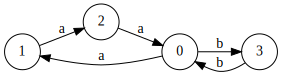
\includegraphics[]{pics/input.pdf}
 \caption{Конечный автомат, задающий регулярную аппроксимацию выражения \textbf{\texttt{expr}}}
 \label{input}
\end{figure}

В результате работы предложенного алгоритма будет получено конечное представление леса разбора SPPF, изображённое на рисунке~\ref{sppf}.

\begin{figure}[!h]
 \centering
 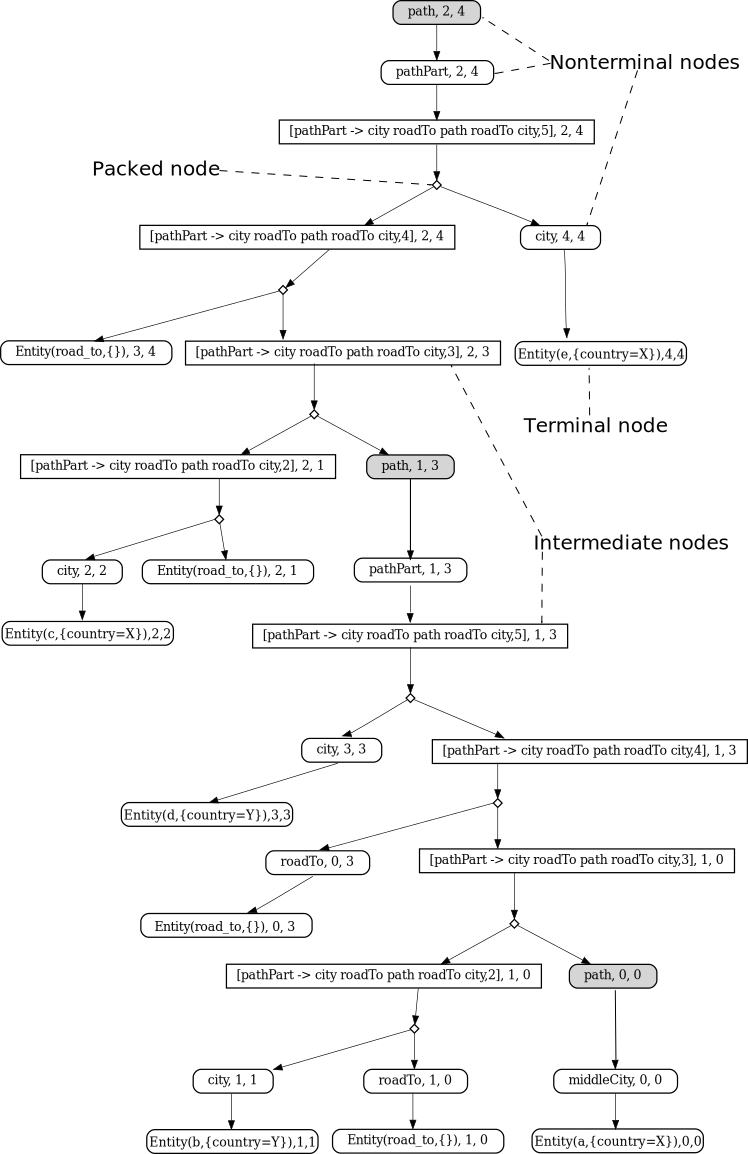
\includegraphics[width=15cm]{pics/sppf.pdf}
 \caption{Конечное представление леса разбора для выражения \textbf{\texttt{expr}}}
 \label{sppf}
\end{figure}

\begin{figure}[!h]
 \centering
 \includegraphics[width=.4\textwidth]{pics/sppf1.pdf}
 \caption{Дерево вывода для выражения $expr="()"$}
 \label{sppf1}
\end{figure}

\begin{figure}[!h]
 \centering
 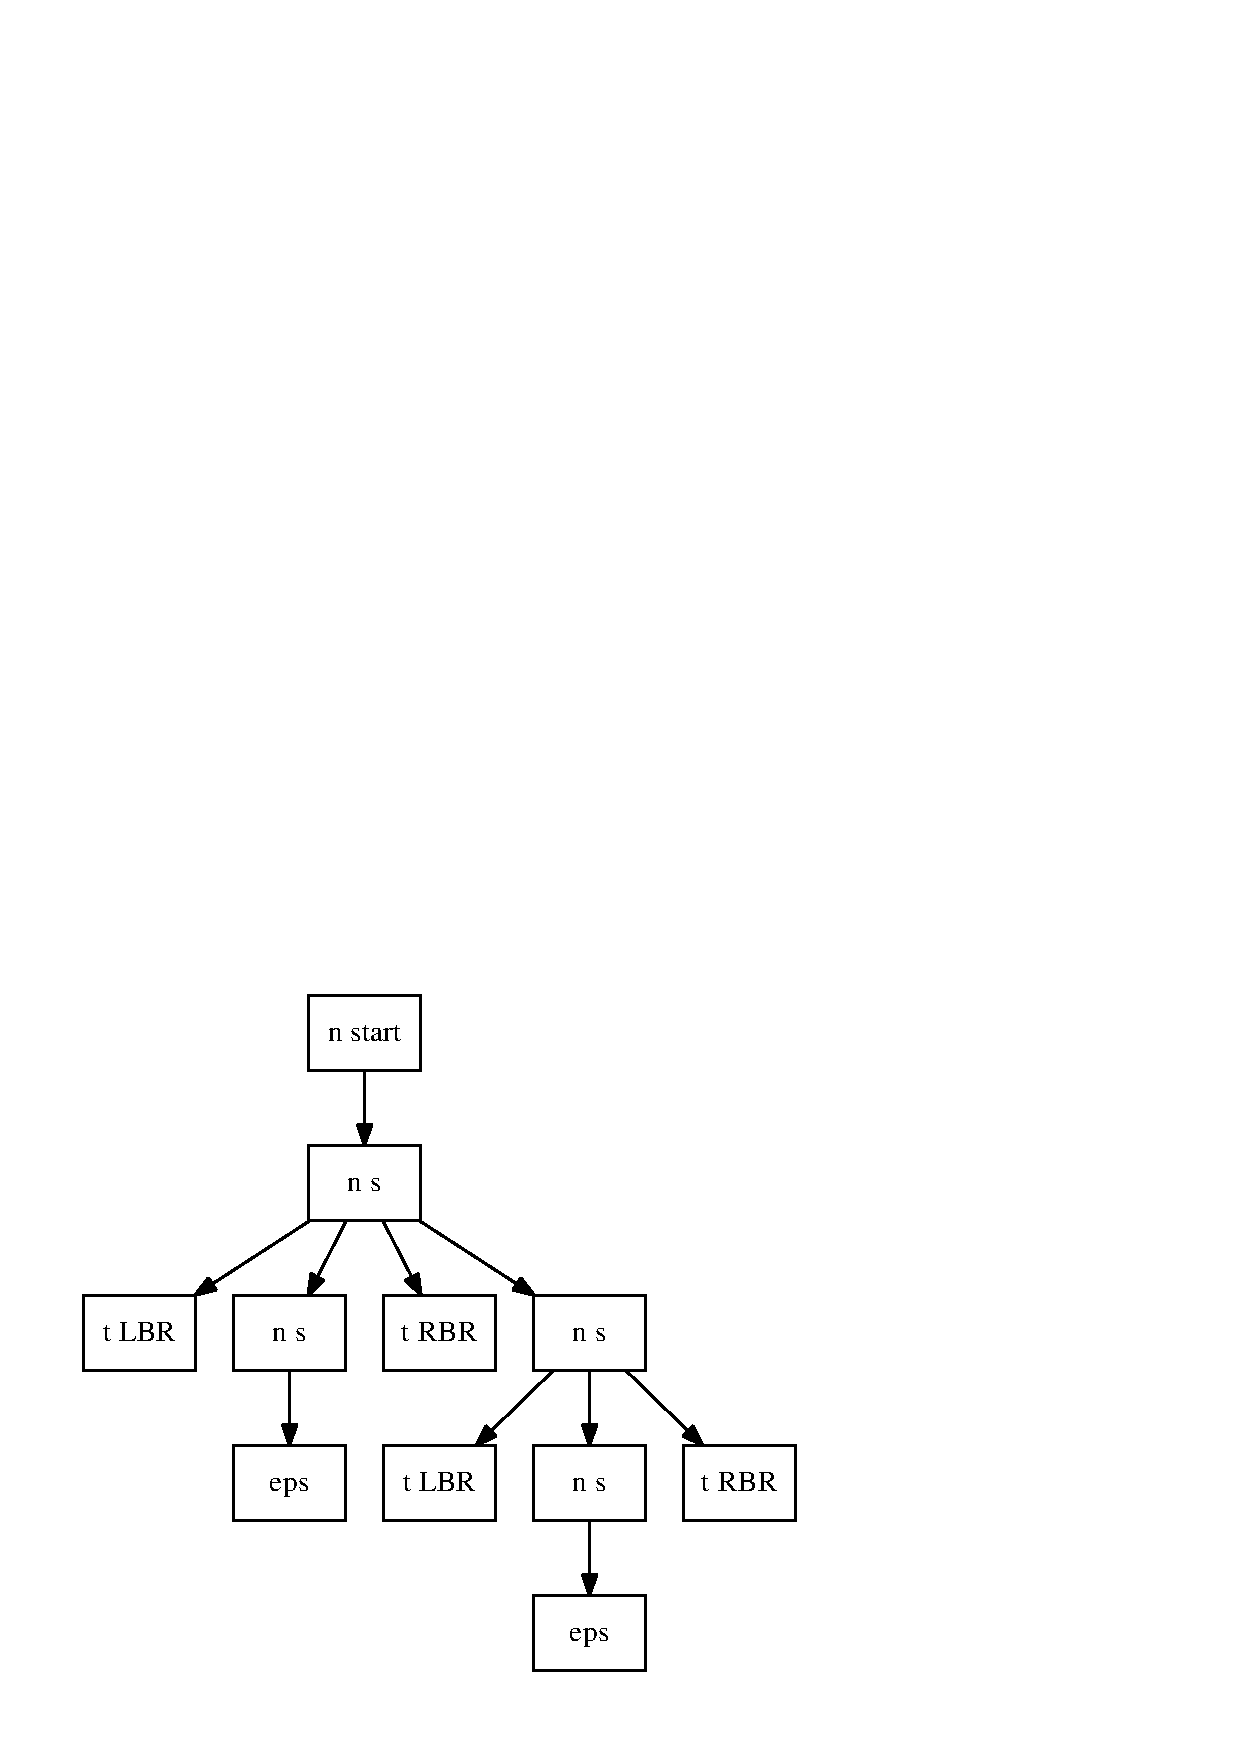
\includegraphics[width=.5\textwidth]{pics/sppf2.pdf}
 \caption{Дерево вывода для выражения $expr="()()"$}
 \label{sppf2}
\end{figure}

\begin{figure}[!h]
 \centering
 \includegraphics[width=.7\textwidth]{pics/sppf3.pdf}
 \caption{Дерево вывода для выражения $expr="()()()"$}
 \label{sppf3}
\end{figure}

Из построенного SPPF можно извлечь бесконечное количество деревьев, каждое из которых является деревом вывода некоторой цепочки из регулярной аппроксимации. На серии рисунков~\ref{sppf1},~\ref{sppf2},~\ref{sppf3} представлены извлечённые деревья разбора для различных значений выражения \textbf{\texttt{expr}}.  


\section{Доказательство корректности алгоритма ослабленного синтаксического анализа регулярной аппроксимации}

\textsc{Теорема 1.} 
\textit{Алгоритм завершает работу для любых входных данных.}

\textsc{Доказательство.}
С каждой вершиной внутреннего представления графа входного конечного автомата ассоциировано не более $N$ вершин графа GSS, где $N$~--- это количество состояний синтаксического анализатора. Таким образом, количество вершин в графе GSS ограничено сверху числом $N \times n$, где $n$~--- это количество вершин графа входного автомата. Так как в GSS нет кратных ребер, количество его ребер~--- $O((N \times n)^{2})$. На каждой итерации основного цикла алгоритм извлекает из очереди $Q$ и обрабатывает одну вершину внутреннего графа. Вершины добавляются в очередь $Q$ только тогда, когда происходит добавление нового ребра в GSS. Так как количество ребер в GSS конечно, алгоритм завершает работу для любых входных данных. $\square$

Для того, чтобы доказать корректность построения конечного представления леса разбора, нам потребуется следующее определение. 

\textsc{Определение 1.} 
\emph{Корректное дерево}~--- это упорядоченное дерево со следующими свойствами.
\begin{enumerate}
  \item Корень дерева соответствует стартовому нетерминалу грамматики $G$.
  \item Листья соответствуют терминалам грамматики $G$. Упорядоченная последовательность листьев соответствует некоторому пути во входном графе.
  \item Внутренние узлы соответствуют нетерминалам грамматики $G$. Дети внутреннего узла (для нетерминала $N$) соответствуют символам правой части некоторой продукции для $N$ в грамматике $G$.
\end{enumerate}

Неформально, корректное дерево~--- это дерево вывода некоторой цепочки из регулярного множества в эталонной грамматике. Далее нам необходимо доказать, во-первых, что конечное представление леса разбора SPPF содержит только корректные деревья, во-вторых, что для каждой корректной относительно эталонной грамматики цепочки существует корректное дерево вывода в SPPF. 

\textsc{Лемма.}
\textit{Пусть обрабатывается внутренний граф $\mathcal{G}=(V,E)$. Тогда для каждого ребра GSS $(v_{t}, v_{h})$ такого, что $v_{t} \in V_{t}.processed$, $v_{h} \in V_{h}.processed$, где $V_{t} \in V$ и $V_{h} \in V$, терминалы ассоциированного поддерева соответствуют некоторому пути из вершины $V_{h}$ в $V_{t}$ в графе $\mathcal{G}$.}

\textsc{Доказательство.}
Будем строить доказательство при помощи индукции по высоте дерева вывода. База индукции --- это минимальное дерево: либо $\varepsilon$-дерево, либо дерево, состоящее из единственной вершины-терминала. При этом $\varepsilon$-дерево соответствует пути длины $0$; начальная и конечная вершины ребра, соответствующего такому дереву, совпадают, поэтому утверждение верно. Дерево, состоящее из одной вершины, соответствует терминалу, считанному с некоторого ребра $(V_{h}, V_{t})$ внутреннего графа, поэтому утверждение верно. 

Корнем дерева высоты $k$ является нетерминал $N$. По третьему пункту определения корректного дерева существует некоторое правило эталонной грамматики $N \rightarrow A_{0}, A_{1}, \dots, A_{n}$, где $A_{0}, A_{1}, \dots, A_{n}$ являются детьми корневого узла. Поддерево $A_{i}$ ассоциированно с ребром $(v_{t}^{i}, v_{h}^{i})$ графа GSS и, так как его высота равна $k-1$, то по индукционному предположению существует путь во внутреннем графе из вершины $V_{h}^{i}$ в вершину $V_{t}^{i}$. Вершина $V_{t}^{i} = V_{h}^{i+1}$, так как $v_{t}^{i} = v_{h}^{i+1}$, поэтому во внутреннем графе существует путь из вершины $V_{h}^{0}$ в вершину $V_{t}^{n}$, соответствующий рассматриваемому корректному дереву. $\square$

Так как SPPF является сжатым представлением леса разбора, то для получения конкретного дерева его необходимо \textit{извлечь} из SPPF.

\textsc{Теорема 2.} 
\textit{Любое дерево, извлечённое из SPPF, является корректным.}

\textsc{Доказательство.}
Рассмотрим произвольное дерево, извлечённое из SPPF, и докажем, что оно удовлетворяет определению 1. Первый и третий пункт определения корректного дерева следует из определения SPPF. Второй пункт определения следует из \textsc{леммы}, если применить её к рёбрам из GSS, начало которых лежит на последнем уровне стека и помечено принимающим состоянием, а конец~--- в вершинах на уровне 0. $\square$

\textsc{Теорема 3.} 
\textit{Для каждой строки, соответствующей пути $p$ во входном графе, и выводимой в эталонной грамматике $G$, из SPPF может быть извлечено корректное дерево $t$. То есть $t$ будет являться деревом вывода цепочки, соответствующей пути $p$, в грамматике $G$.}

\textsc{Доказательство.}
Рассмотрим произвольное корректное дерево и докажем, что оно может быть извлечено из SPPF. Доказательство повторяет доказательство корректности для RNGLR-алгоритма~\cite{RNGLR}, за исключением следующей ситуации. RNGLR-алгоритм строит граф GSS по слоям: гарантируется, что $\forall j \in [0..i-1], j-$ый уровень GSS будет зафиксирован на момент построения $i-$ого уровня. В нашем случае это свойство не верно, так как во входном графе могут быть циклы и нет возможности упорядочить обработку его вершин. Это, в свою очередь, может приводить к появлению новых путей для свёрток, которые уже были ранее обработаны. Единственный возможный способ образования такого нового пути~--- это добавление ребра $(v_{t}, v_{h})$, где вершина $v_{t}$ ранее присутствовала в GSS и имела входящие ребра. Так как алгоритм сохраняет информацию о том, какие свёртки проходили через вершины GSS, то достаточно продолжить свёртки, проходящие через вершину $v_{t}$. Таким образом гарантируется выполнение всех возможных свёрток и построение корректного дерева вывода. $\square$

\textsc{Замечание.} Построение леса разбора осуществляется одновременно с построением GSS, при этом дерево вывода нетерминала связывается с ребром GSS каждый раз при обработке соответствующей свёртки, вне зависимости от того, было ли ребро в графе до этого или добавлено на данном шаге. Это обстоятельство позволяет утверждать, что если все возможные редукции были выполнены, то и лес разбора содержит все деревья для всех корректных цепочек из аппроксимации.

\chapter{Инструментальный пакет} \label{relWorks}

В данной главе описан инструментальный пакет (Software Development Kit, SDK) \textbf{YC.SEL.SDK}, предназначенный для разработки различных решений по статическому анализу динамически формируемых выражений. Представлена архитектура разработанного SDK, а также архитектура надстройки \textbf{YC.SEL.SDK.ReSharper}, позволяющей создавать расширения для ReSharper, предоставляющие поддержку встроенных языков. Изложенный выше алгоритм синтаксического анализа реализован в рамках одной из компонент SDK. YC.SEL.SDK и YC.SEL.SDK.ReSharper являются \textbf{платформами} для разработки инструментов статического анализа динамически формируемого кода.

\section{Архитектура}

Практически любой язык программирования может использоваться как встроенный. Даже если рассматривать только SQL, то окажется, что у него множество различных диалектов, каждый из которых имеет свои особенности. Внешним языком также может быть любой язык программирования. Трудность заключается в том, что  любое из сочетаний внешнего и встроенного языка может встретиться на практике, и задачи, которые необходимо решать в этой ситуации, могут быть различными (поиск ошибок, подсчёт метрик, автоматизация трансформаций и т.д.). Реализовать универсальный инструмент, решающий все задачи для всех языков, не представляется возможным. Более целесообразно создать набор инструментов, упрощающий создание конечных решений для конкретных языков и конкретных задач. В качестве примера можно рассмотреть инструменты для разработки компиляторов, которые включают в себя генераторы лексических, синтаксических анализаторов и набор библиотек с вспомогательными функциями, и тем самым упрощают создание конкретного компилятора для выбранного языка и целевой платформы.

Требуемый набор инструментов для работы со встроенными языками должен поддерживать весь процесс обработки кода, который может выглядеть так, как представлено на рисунке~\ref{fig:SeqSelProcessing}. Можно выделить следующие основные шаги.
\begin{itemize}
    \item Анализ основного кода, который выполняется сторонним инструментом. Результат этого шага --- это дерево разбора с информацией, достаточной для выполнения дальнейших шагов.
    \item Построение аппроксимации множества возможных значений динамически формируемых выражений.
    \item Лексический анализ построенной на предыдущем шаге аппроксимации.
    \item Синтаксический анализ, результатом которого является лес разбора, пригодный для дальнейшей обработки.
    \item Обработка леса разбора, вычисление семантики.
\end{itemize}

На каждом шаге может быть получена информация, полезная для пользователя, такая как список ошибок, и её необходимо отобразить для него соответствующим образом.

\begin{figure}[h!]
\begin{center}
\includegraphics[width=0.9\textwidth]{pics/Activ_SEL_Processing}
\caption{Диаграмма последовательности обработки встроенных языков}
\label{fig:SeqSelProcessing} 
\end{center}
\end{figure}


Существующие инструменты для работы со встроенными языками обычно реализуют поддержку какого-то фиксированного набора языков. При этом поддержка нового языка, как правило, требует нетривиальнй доработки инструмента. Чтобы получить поддержку встроенного языка без изменений в исходном коде базового инструмента, необходимо предоставить соответствующий механизм. 

Для того чтобы упростить процесс создания конечных инструментов, создан SDK, одной из компонент которого является генератор синтаксических анализаторов на основе предложенного в данной работе алгоритма. Также в него входит генератор лексических анализаторов, библиотека построения регулярной аппроксимации, набор вспомогательных функций. Подробное описание компонент приведено далее.

Так как анализ внешнего языка является сложной самостоятельной задачей, то он не включён в разработанный SDK. На вход созданному на основе SDK инструменту должно подаваться дерево разбора внешнего языка с информацией, достаточной для решения поставленных в данной работе задач. 


\subsection{Архитектура YS.SEL.SDK}

Разработанный SDK включает компоненты, необходимые для реализации шагов, представленных на рисунке ~\ref{fig:SeqSelProcessing} и описанных ранее, за исключением анализа внешнего языка. Архитектура SDK изображена на рисунке~\ref{fig:SDKHLArch} и включает в себя генераторы анализаторов и различные библиотеки времени исполнения.

\begin{figure}[h!]
\begin{center}
\includegraphics[width=0.9\textwidth]{pics/HighLevelArch}
\caption{Архитектура SDK целиком}
\label{fig:SDKHLArch} 
\end{center}
\end{figure}

Так как анализ внешнего языка не входит в задачи разработанного SDK, то первый шаг, выполнение которого необходимо обеспечить, --- это построение аппроксимации. В нашем случае строится регулярное приближение множества значений динамически формируемого выражения.

Построение регулярной аппроксимации основано на алгоритме, изложенном в работе~\cite{RegOverApprox}, который позволяет строить приближение сверху для множества значений выражений. То есть $L_R$, задаваемый регулярным приближением, не меньше, чем $L_1$, задаваемый программой (выполняется включение $L_R \in L_1$). Это позволяет говорить о надёжности дальнейших анализов в том смысле, что они не теряют информации о $L_1$. Например, это важно при поиске ошибок. Если в $L_R$ не обнаружено ошибок (то есть $L_R \in L_2$, где $L_2$ --- эталонный), значит и в $L_1$ ошибок нет. При этом могут быть найдены ошибки в $L_R$, которых нет в $L_1$, то есть будут ложные срабатывания. Однако наличие ложных срабатываний лучше, чем пропущенные ошибки, и их количество может быть уменьшено путём повышения точности аппроксимации. 

Для того чтобы сделать построение приближения независимым от внешнего языка, реализовано обобщённое представление графа потока управления (Control Flow Graph, CFG)~\cite{Dragon}, которое содержит всю необходимую для дальнейшей работы информацию. Таким образом, разработчику необходимо реализовать построение обобщённого представления CFG для конкретного внешнего языка. В результате компонента строит конечный автомат, являющийся приближением множества значений динамически формируемых выражений.

Компонента, отвечающая за лексический анализ, состоит из двух частей: генератора лексических анализаторов, который по описанию лексики обрабатываемого языка строит соответствующий конечный преобразователь, и интерпретатора, который производит анализ входной структуры данных на основе построенного генератором преобразователя. Архитектура компоненты представлена на рисунке~\ref{fig:LexArch}. На вход принимается конечный автомат над символами, результатом работы является конечный автомат над алфавитом токенов анализируемого языка. Входной конечный автомат может быть построен с помощью компоненты построения регулярной аппроксимации. Основные структуры данных --- конечный автомат и конечный преобразователь --- и функции работы с ними описаны в соответствующей библиотеке.

\begin{figure}[h!]
\begin{center}
\includegraphics[width=0.95\textwidth]{pics/LexerDiagram}
\caption{Архитектура лексического анализатора}
\label{fig:LexArch} 
\end{center}
\end{figure}

Лексический анализатор реализован на основе инструмента FsLex, который является стандартным генератором лексических анализаторов для языка F\#. При реализации был переиспользован язык описания лексики и некоторые структуры данных.

Реализованный генератор лексических анализаторов обладает следующими особенностями.
\begin{itemize}
    \item Поддерживаются разрывные токены, то есть токены формируемые из нескольких строковых литералов.
    \item Сохраняется привязка лексических единиц к исходному коду: сохраняется информация о строковом литерале, из которого породился токен и координаты его внутри этой строки. Так как одна лексическая единица может формироваться из нескольких строковых литералов, то привязка сохраняется отдельно для каждой части.
    \item Поддерживается обработка входных конечных автоматов, содержащих циклы.
    \item Так как значение токена может формироваться с помощью цикла и, как следствие, быть бесконечным, то каждый токен содержит конечный автомат, порождающий все возможные значения для данного токена, а не единственное значение, как это реализовано в классическом лексическом анализе.
\end{itemize}

\textbf{Генератор синтаксических анализаторов}, названный ARNGLR, реализован на основе алгоритма, описанного в разделе~\ref{AlgoDescr}. Его архитектура представлена на рисунке~\ref{fig:ParsArch}.  

\begin{figure}[h!]
\begin{center}
\includegraphics[width=0.95\textwidth]{pics/ARNGLRArch}
\caption{Архитектура синтаксического анализатора}
\label{fig:ParsArch} 
\end{center}
\end{figure}

Генератор реализован как один из модулей YC и может принимать на вход внутреннее представление грамматики (IL), которое может быть получено с помощью различных фронтендов (Frontends), однако в рамках YC.SEL.SDK 
основным фронтендом является YARD, так как он предоставляет наиболее развитые средства для описания грамматик. По грамматике обрабатываемого языка строятся управляющие таблицы анализатора, которые сохраняются в файле Parser.fs. 
Построенные таблицы должны быть включены в разрабатываемое приложение UserApplication. Интерпретатор, предназначенный для синтаксического разбора конечного автомата, полученный после лексического анализа, реализован 
в виде отдельной библиотеки ARNGLR.Runtime, которая также должна быть подключена к разрабатываемому приложению. В результате работы интерпретатора будет получен SPPF, который может быть использован для дальнейшей 
обработки (например, подсчёта метрик). Для упрощения работы с SPPF реализован ряд вспомогательных функций.

\subsection{Архитектура YC.SEL.SDK.ReSharper}

ReSharper --- это расширение к Microsoft Visual Studio IDE, предоставляющее широкий спектр  дополнительной функциональности по анализу и рефакторингу кода. ReSharper поддерживает несколько языков, например C\#, Visual Basic .NET, JavaScript, и этот список может быть расширен благодаря наличию свободно распространяемого ReSharper SDK, описание которого было представлено ранее в разделе~\ref{ReSharperSDKDescr}. ReSharper.SDK позволяет получить деревья разбора для поддерживаемых языков, предоставляет набор готовых анализов и упрощает взаимодействие с Microsoft Visual Studio IDE и её компонентами. Более того, предоставляется возможность разработки собственных расширений для ReSharper на основе ReSharper.SDK.

Microsoft Visual Studio является достаточно распространённой средой разработки, но не поддерживает встроенные языки, поэтому было решено разработать ряд расширений к ReSharper с использованием разработанного инструментария, которые будут устранять данный недостаток. Стоит отметить, что не ставилось задачи поддержать все встроенные языки, так как встроенным может быть любой язык программирования. Также не было необходимости поддержать все внешние языки программирования. Необходимо на базе разработанного YC.SEL.SDK создать инфраструктуру, позволяющую реализовывать поддержку новых встроенных языков в Microsoft Visual Studio через расширения к ReSharper и реализовать несколько расширений, демонстрирующих возможности созданной инфраструктуры. 

Так как необходимо поддерживать различные языки, то необходимо обеспечить расширяемость по новыми языками. Классический подход к решению такой задачи для интегрированных сред разработки заключается в том, что поддержка нового языка реализуется в виде независимой компоненты. Если пользователь хочет получить поддержку какого-либо языка в своей среде разработки, то он должен установить соответствующий пакет. При этом поддержка различных языков осуществляется независимо, однако часто выделяется общая функциональность, которая может быть оформлена в виде отдельного пакета.

Для предоставления описанных выше возможностей была реализована надстройка над YC.SEL.SDK, упрощающая создание расширений для ReSharper, названная  YC.SEL.SDK.ReSharper. В неё включены компоненты, реализующие функции, которые упрощающают взаимодействие YC.SEL.SDK и ReSharper.SDK. Назначени основных из них описаны ниже.

\begin{itemize}
  \item Общая точка расширения, необходимая для подключения функциональности для различных встроенных языков, которая может быть реализована в различных расширениях, к ReSharper через общий интерфейс. Также общая точка расширения позволяет использовать общую функциональность, необходимую для работы со встроенными языками.
  \item Отображение в IDE информации, полученной в ходе анализа. Например, подсветка синтаксиса и ошибок. Вывод диагностических сообщений с информацией об ошибках.
  \item Преобразование данных, из формата, используемого в ReSharper.SDK, в формат для YC.SEL.SDK. Например, преобразование графа потока управления внешнего языка, построенного ReSharper.SDK, в формат, пригодный для построения регулярной аппроксимации средствами YC.SEL.SDK.
  \item Управление работой анализаторов, необходимое, с одной стороны, для обеспечения своевременной реакции на изменения в коде, совершённые пользователем, а с другой, для прекращения вычислений, результаты которых уже не актуальны. Управление построено на основе общего для ReSharper механизма, обеспечивающего асинхронную работу анализов. При этом вычисления могут быть прерваны, если, например, пользователь внёс в код изменения, делающие анализ или его результаты некорректными. 
\end{itemize}

Как уже говорилось, встроенными могут быть различные языки и учесть заранее все их особенности не представляется возможным. Кроме того, даже при использовании одного встроенного языка могут использоваться различные способы выполнения сформированного запроса. Таким образом, необходимо предоставлять возможность настройки расширений конечным пользователем. Для этого в рамках YC.SEL.SDK.ReSharper была реализована возможность управления следующими основными параметрами расширений. 

\begin{itemize}
    \item Подсветка синтаксиса для каждого языка. Предоставлена возможность указать цвет для каждого типа токена.
    \item Указание парных элементов. Для каждого языка можно указать, какие лексические единицы считать парными: для каждой пары указывается ``левый'' (открывающая скобка) и ``правый'' (закрывающая скобка) элементы. При расположении курсора в тексте рядом с одним из элементов пары будут подсвечены соответствующие элементы. Пример подсветки парных элементов приведён на рисунке~\ref{fig:braces}.
    \item Точки интереса или хотспоты (hotspot) --- это места, в которых должно быть сформировано финальное выражение. Необходимо знать, какой хотспот какому языку соответствует. При этом нужно учитывать, что одному языку может соответствовать несколько хотспотов. Например, динамически сформированный SQL-запрос в программе на языке программирования C\# может быть выполнен с помощью метода \verb|ExecuteQuery| класса \verb|DataContext|~\cite{ExecuteQuery}
     или же текст запроса может быть передан как аргумент конструктора класса \verb|SqlCommand|~\cite{SqlCommand} с последующим выполнением с помощью метода \verb|ExecuteReader|.

\end{itemize}

Настройка указанных выше параметров хранится в соответствующих конфигурационных файлах в формате XML, которые на данный момент редактируются вручную. Настройка подсветки синтаксиса и парных элементов совмещена в одном файле и для каждого языка создаётся отдельный такой файл. Конфигурационный файл с точками интереса является общим для всех языков и, соответственно, для всех установленных расширений для поддержки встроенных языков.

В листинге~\ref{lst:codeHighlighting} приведён пример конфигурации подсветки синтаксиса и парных скобок для языка Calc. Для указания цвета используются имена, принятые в ReSharper (например, \verb|"CONSTANT_IDENTIFIER_ATTRIBUTE"|), что должно сделать настройку цветов более единообразной. В xml-тэге \verb|Matched| содержится описание парных элементов. Каждая пара описывается в xml-тэге \verb|Pair| и для одного языка может быть указано более одной такой пары.

\fvset{frame=lines,framesep=5pt}
\begin{listing}[H]
    \begin{pyglist}[language=xml,numbers=left,numbersep=5pt]
<?xml version="1.0" encoding="utf-8"?>
<SyntaxDefinition name="CalcHighlighting">
    <Colors>
        <Tokens color="CONSTANT_IDENTIFIER_ATTRIBUTE">
            <Token> DIV </Token>
            <Token> LBRACE </Token>
            <Token> MINUS </Token>
            <Token> MULT </Token>
            <Token> NUMBER </Token>
            <Token> PLUS </Token>
            <Token> POW </Token>
            <Token> RBRACE </Token>
        </Tokens>
    </Colors>
<!-- Dynamic highlighting: -->
    <Matched>
        <Pair>
            <Left> LBRACE </Left>
            <Right> RBRACE </Right>
        </Pair>
<!-- You can specify more then one pair:        
        <Pair>
            <Left> LEFT_SQUARE_BRACKET </Left>
            <Right> RIGHT_SQUARE_BRACKET </Right>
        </Pair>
        <Pair>
            <Left> LEFT_FIGURE_BRACKET </Left>
            <Right> LEFT_FIGURE_BRACKET </Right>
        </Pair>
-->        
    </Matched>
</SyntaxDefinition>
    \end{pyglist}
\caption{Пример конфигурационного файла для настройки подсветки синтаксиса}
\label{lst:codeHighlighting}
\end{listing}

Листинг~\ref{lst:hotspots} содержит пример описания точек интереса. Для каждой точки интереса должна быть указана следующая информация.
\begin{itemize}
    \item Какому встроенному языку соответствует точка. Информация хранится в Xml-тэге \verb|Language|.
    \item Полное имя метода, являющегося точкой интереса. Информация хранится в Xml-тэге \verb|Method|.
    \item Порядковый номер аргумента данного метода, являющегося выражением на встроенном языке. Нумерация начинается с нуля. Информация хранится в Xml-тэге \verb|ArgumentPosition|. 
    \item Возвращаемый тип метода.  Информация хранится в Xml-тэге \verb|ReturnType|. 
\end{itemize}

\fvset{frame=lines,framesep=5pt}
\begin{listing}[H]
    \begin{pyglist}[language=xml,numbers=left,numbersep=5pt]
<?xml version="1.0" encoding="utf-8"?>
<!-- comment about body -->
<Body>
    <!-- comment about hotspot -->
  <Hotspot>
      <!-- comment about tsql -->
      <Language> TSQL </Language>
      <!-- comment about fullName -->
      <Method>Program.ExecuteImmediate</Method>
      <!-- zero-based -->
      <ArgumentPosition> 0 </ArgumentPosition>
      <!-- comment about return type -->
      <ReturnType> void </ReturnType>
  </Hotspot>
  <Hotspot>
      <Language> Calc </Language>
      <Method>Program.Eval</Method>
      <ArgumentPosition> 0 </ArgumentPosition>
      <ReturnType> int </ReturnType>
  </Hotspot>
</Body>
    \end{pyglist}
\caption{Пример конфигурационного файла для настройки точек интереса}
\label{lst:hotspots}
\end{listing}


\section{Области и способы применения YC.SEL.SDK}

Разработанный SDK предназначен для создания инструментов статического анализа динамически формируемых строковых выражений. Решения, созданные с его помощью, могут применяться для работы с проектами, активно использующими динамически формируемые строковые выражения. Необходимость работать с такими проектами может возникнуть, например, в следующих областях.

\begin{itemize}
    \item Реинжиниринг программного обеспечения.
    \item Поддержка встроенных языков в средах разработки.
    \item Оценка качества и сложности кода.
\end{itemize}

Общим для всех этих областей является то, что для решения многих задач необходимо структурное представление динамически формируемого кода. При этом анализируемые языки могут быть различными и процесс их анализа часто тесно связан с анализом внешнего языка.

Отметим, что встроенные языки используются всё менее активно в молодых проектах и системах. На смену им приходят более надёжные способы композиции языков и метапрограммирования. Например LINQ или ORM-технологии. Однако это не всегда так. Использование строковых выражений для взаимодействия с базами данных и генерации WEB-страниц в приложениях на PHP всё ещё широко распространено~\cite{DSQLInActiveUse}. Это необходимо учитывать при поддержке встроенных языков в средах разработки. Для каких-то языков на первый план выходят возможности по изучению и модификации уже созданного кода, а для каких-то --- возможность быстро и удобно создавать новый код. Во втором случае могут возникнуть дополнительные требования к скорости работы инструмента, так как подразумевается выполнение некоторых операций ``на лету'', что может послужить ограничением на использование SDK, так как многие механизмы, реализованные в нём, не предусматривают возможности уменьшения точности в пользу увеличения быстродействия. Оценка качества и сложности  кода часто может выполняться в рамках комплекса задач по реинжинирингу системы, однако может быть и самостоятельной задачей, например, при оценке сложности работ по поддержке и сопровождению информационной системы.

Детали применения SDK могут варьироваться в зависимости от решаемых задач и контекста использования. Например, механизм построения регулярной аппроксимации может быть реализован независимо в рамках внешнего инструмента. Однако основной сценарий использования аналогичен использованию инструментариев для разработки компиляторов. Последовательность шагов, представленная ниже, может быть изменена в зависимости от особенностей задачи.

\textbf{Шаг 1.} Создание грамматики обрабатываемого языка. Грамматика может быть создана на основе документации соответствующего языка или переиспользована готовая, что оправданно, например, при создании анализатора для динамического SQL, когда внешний и встроенный языки совпадают.

\textbf{Шаг 2.} Генерация синтаксического анализатора по созданной грамматике. Для этого используется генератор синтаксических анализаторов, присутствующий в SDK. Результатом работы генератора является файл с исходным кодом на языке программирования F\#, который должен быть включён в разрабатываемый код. Файл содержит описание типов для лексических единиц, управляющие таблицы анализатора и функцию, которая по конечному автомату над алфавитом токенов анализируемого языка построит SPPF, содержащий деревья вывода всех корректных цепочек.

\textbf{Шаг 3.} Создание лексической спецификации обрабатываемого языка. Спецификация может быть извлечена из документации или заимствована из других проектов. При обработке динамически формируемого SQL возможно переиспользовать спецификацию, созданную для основного языка, которым также является SQL. При этом необходимо обратить внимание на то, что типы лексических единиц определяются на основе созданного на предыдущих шагах синтаксического анализатора.

\textbf{Шаг 4.} Генерация лексера по созданной спецификации. Для этого применяется генератор лексических анализаторов, входящий в состав SDK. В результате его применения получается файл с исходным кодом на языке F\#, который должен быть подключён к разрабатываемому решению. 

\textbf{Шаг 5.} Реализация механизма построения регулярной аппроксимации, результатом которого является функция, строящая конечный автомат над алфавитом символов. Данный механизм может быть реализован либо на основе предоставляемого в рамках SDK, либо независимо. В первом случае от разработчика требуется построить обобщённый CFG для внешнего языка. Во втором случае необходимо только гарантировать правильность возвращаемого конечного автомата. Второй подход может быть использован, например, при наличии реализованного механизма протягивания констант для внешнего языка. Это позволит создать возможно менее точное, но, скорее всего, более быстрое построение аппроксимации. Такой подход применим при автоматизированном реинжиниринге, когда ручная доработка кода является обязательным шагом и абсолютная точность автоматической обработки не требуется. Ещё одна возможная область применения второго подхода --- это поддержка встроенных языков в средах разработки. Здесь также часто не требуется высокая точность для подсказок пользователю, однако производительность крайне важна. Поэтому иногда приходится жертвовать точностью анализа для достижения нужной скорости работы.

\textbf{Шаг 6.} Реализация работы с SPPF. Синтаксический анализатор возвращает SPPF --- конечное представление леса разбора всех корректных цепочек из аппроксимации. Дальнейшая работа с ним может строиться по двум основным сценариям.

Превый сценарий --- непосредственная обработка SPPF. В этом случае все вычисления происходят над SPPF без извлечения отдельных деревьев. Это позволит ускорить обработку результатов разбора, так как количество деревьев может быть бесконечным, а SPPF является конечной структурой данных. Однако существует несколько проблем, связанных с таким подходом. Во-первых, требуется создание новых процедур обработки, так как классические, как правило, ориентированы на работу с деревьями. Во-вторых, могут возникнуть трудности при выполнении некоторых анализов, вызванные тем, что в SPPF хранятся ``бесконечные'' деревья. Например, необходимо вычислить максимальную глубину вложенности конструкции \verb|if|, являющуюся одной из стандартных метрик сложности кода. SPPF может содержать 
циклы и может оказаться так, что конструкция \verb|if| встречается в цикле таким образом, что потенциальная глубина вложенности может быть бесконечной. Такая ситуация не является стандартной при 
обработке деревьев разбора и её надо отслеживать отдельно.

Второй сценарий --- извлечение отдельных деревьев из SPPF и их обработка. Данный подход может оказаться удобным, если уже существуют процедуры обработки синтаксических деревьев для языка, который оказался встроенным. Это помогает избежать затрат на создание новой функциональности. Такое может произойти при работе с динамическим SQL. В этом случае для работы с деревом разбора внешнего языка и деревьями, извлечёнными из SPPF, можно использовать одни и те же процедуры, так как языки идентичны.

Недостатком второго подхода является то, что конечность числа деревьев не гарантирована. Это значит, что не удастся обработать все деревья. Стоит отметить, что даже в случае конечности числа деревьев, перебор и обработка всех деревьев разбора может потребовать значительных ресурсов.


\textbf{Шаг 7.} Реализация механизмов сбора, обработки и отображения информации, такой как сообщения об ошибках или любой другой, полученной в процессе анализа. Необходимо для предоставления пользователю информации, ожидаемой в рамках решаемой задачи.

На рисунке~\ref{fig:activMethod} изображён один из возможных сценариев использования SDK. Особенностью является цикличность процесса, характерная, например для реинжиниринга программного обеспечения.

\begin{figure}[h!]
\begin{center}
\includegraphics[width=0.9\textwidth]{pics/ActivMethodology}
\caption{Один из возможных вариантов использования SDK в проектах по реинжинирингу}
\label{fig:activMethod} 
\end{center}
\end{figure}

Встраивание анализа строковых выражений в последовательность обработки кода всей системы зависит от решаемых задач. Первыми шагами идут действия, необходимые для того, чтобы получить входные данные для анализа. Для этого необходимо провести лексический и синтаксический анализ внешнего языка, построить граф потока управления. После этого возможно построение аппроксимации и дальнейший анализ встроенных языков. Параллельно с этим может проводиться дальнейшая обработка внешнего языка. Степень параллельности зависит от независимости решаемых задач. Например, некоторые метрики сложности для основного кода и для динамически формируемого можно считать независимо и выводить отдельно. С другой стороны, может возникнуть необходимость вычислить некую комплексную метрику, учитывающую параметры и внешнего и динамически формируемого кода, что приведёт к необходимости синхронизации.

\section{Особенности реализации}

Разработка инструментального пакета с описанной выше архитектурой и плагинов для ReSharper велась в рамках исследовательского проекта YaccConstructor (YC), описанного в разделе~\ref{YCDescr}. 
Разработка велась на платформе .NET и основной язык реализации --- F\#~\cite{FSharp}. Весь исходный код опубликован на GitHub~\cite{YCUrl}. 
Большинство компонент опубликовано под ``открытой'' лицензией Apache License Version~2.0~\cite{ApacheV2}. 

За основу алгоритма синтаксического анализа динамически формируемых выражений был взят реализованный в YC алгоритм синтаксического анализа RNGLR. Генератор управляющих таблиц был использован практически без 
модификаций, а интерпретатор был реализован отдельный. Кроме этого, общими являются некоторые структуры данных и вспомогательные функции, такие как представление леса разбора и его печать в формате 
DOT~\footnote{DOT --- текстовый язык описания графов~\cite{DOT}.}, представление GSS. 

Лексичекий анализ реализован на основе инструмента FsLex, который потребовал значительных доработок для того, чтобы обеспечить обработку конечного автомата, а не линейного входа. Все остальные компоненты, 
необходимые для статического анализа динамически формируемых выражений, такие как построение аппроксимации, вспомогательные функции для упрощения построения целевых инструментов были реализованы ``с нуля'' 
в рамках проекта YC.

Бинарные пакеты, содержащие основную функциональность, опубликованы в сети интернет на NuGet~\footnote{NuGet --- менеджер пакетов для платформы .NET и одноимённый ресурс для их публикации. Позволяет публиковать 
и устанавливать пакеты, автоматически отслеживать зависимости между ними~\cite{NuGet}.}.

\chapter{Методика использования}

В данной главе будет изложена методика применения разработанного SDK, представлены области применения, описаны основные шаги использования SDK и их результаты.

\section{Области применения}

Разработанный инструментальный пакет предназначен для создания инструментов статического анализа динамически формируемых строковых выражений. Решения, созданные с помощью описанного SDK, могут использоваться для работы с проектами, активно использующими динамически формируемые строковые выражения, и применяться в следующих областях.

\begin{itemize}
    \item Реинжиниринг программного обеспечения.
    \item Поддержка встроенных языков в средах разработки.
    \item Оценка качества и сложности кода.
\end{itemize}

Общим для всех этих областей является то, что для решения многих задач необходимо структурное представление динамически формируемого кода. При этом анализируемые языки могут быть различными и процесс их анализа часто тесно связан с анализом внешнего языка.

Отметим, что встроенные языки используются всё менее активно в молодых проектах и системах. На смену им приходят более надёжные способы композиции языков и метапрограммирования. Например LINQ или ORM-технологии. Однако это не всегда так. Использование строковых выражений для взаимодействия с базами данных и генерации WEB-страниц в приложениях на PHP всё ещё широко распространено. Это необходимо учитывать при поддержке встроенных языков в средах разработки. Для каких-то языков на первый план выходят возможности по изучению и модификации уже созданного кода, а для каких-то --- возможность быстро и удобно создавать новый код. Во втором случае могут возникнуть дополнительные требования к скорости работы инструмента, так как подразумевается выполнение некоторых операций ``на лету'', что может послужить ограничением на использование SDK, так как многие механизмы, реализованные в нём, не предусматривают возможности уменьшения точности в пользу увеличения быстродействия.

Оценка качества и сложности  кода часто может выполняться в рамках комплекса задач по реинжинирингу системы, однако может быть и самостоятельной задачей, например, при оценке сложности работ по поддержке и сопровождению информационной системы.


\section{Способы применения}

Детали применения SDK могут варьироваться в зависимости от решаемых задач и контекста использования. Например, механизм построения регулярной аппроксимации может быть реализован независимо в рамках внешнего инструмента. Однако основной сценарий использования аналогичен использованию инструментариев для разработки компиляторов. Последовательность шагов, представленная ниже может быть изменена в зависимости от особенностей задачи.

\begin{itemize}
    \item Создание грамматики обрабатываемого языка. Грамматика может быть создана на основе документации соответствующего языка или переиспользована готовая, что оправданно, например, при создании анализатора для динамического SQL, когда внешний и встроенный языки совпадают.
    \item Генерация синтаксического анализатора по созданной грамматике. Для этого используется генератор синтаксических анализаторов, присутствующий в SDK. Результатом работы генератора является файл с исходным кодом на языке программирования F\#, который должен быть включён в разрабатываемый код. Файл содержит описание типов для лексических единиц, управляющие таблицы анализатора и функцию, которая по конечному автомату над алфавитом токенов анализируемого языка построит SPPF, содержащий деревья вывода всех корректных цепочек.
    \item Создание лексической спецификации обрабатываемого языка. Спецификация может быть извлечена из документации или заимствована из других проектов. При обработке динамически формируемого SQL возможно переиспользовать спецификацию, созданную для основного языка, которым также является SQL. При этом необходимо обратить внимание на то, что типы лексических единиц определяются на основе созданного на предыдущих шагах синтаксического анализатора.
    \item Генерация лексера по созданной спецификации. Для этого применяется генератор лексических анализаторов, входящий в состав SDK. В результате его применения получается файл с исходным кодом на языке F\#, который должен быть подключён к разрабатываемому решению. 
    \item Реализация механизма построения регулярной аппроксимации, результатом которого является функция, строящая конечный автомат над алфавитом символов. Данный механизм может быть реализован либо на основе предоставляемого в рамках SDK, либо независимо. В первом случае от разработчика требуется построить обобщённый CFG для внешнего языка. Во втором случае необходимо только гарантировать правильность возвращаемого конечного автомата. Второй подход может быть использован, например, при наличии реализованного механизма протягивания констант для внешнего языка. Это позволит создать возможно менее точное, но, скорее всего, более быстрое построение аппроксимации. Такой подход применим при автоматизированном реинжиниринге, когда ручная доработка кода является обязательным шагом и абсолютная точность автоматической обработки не требуется. Ещё одна возможная область применения второго подхода --- это поддержка встроенных языков в средах разработки. Здесь также часто не требуется высокая точность для подсказок пользователю, однако производительность крайне важна. Поэтому иногда приходится жертвовать точностью анализа для достижения нужной скорости работы.
    \item Реализация работы с SPPF. Синтаксический анализатор возвращает SPPF --- конечное представление леса разбора всех корректных цепочек из аппроксимации. Дальнейшая работа с ним может строиться по двум основным сценариям.
    \begin{itemize}
        \item Непосредственная обработка SPPF. В этом случае все вычисления происходят над SPPF без извлечения отдельных деревьев. Это позволит ускорить обработку результатов разбора, так как количество деревьев может быть бесконечным, а SPPF является конечной структурой данных. Однако существует несколько проблем, связанных с таким подходом. Во-первых, требуется создание новых процедур обработки, так как классические, как правило, ориентированы на работу с деревьями. Во-вторых, могут возникнуть трудности при выполнении некоторых анализов, вызванные тем, что в SPPF хранятся ``бесконечные'' деревья. Например, необходимо вычислить максимальную глубину вложенности конструкции \verb|if|, являющуюся одной из стандартных метрик сложности кода. SPPF может содержать 
циклы и может оказаться так, что конструкция \verb|if| встречается в цикле таким образом, что потенциальная глубина вложенности может быть бесконечной. Такая ситуация не является стандартной при 
обработке деревьев разбора и её надо отслеживать отдельно.
        \item Извлечение отдельных деревьев из SPPF и их обработка. Данный подход может оказаться удобным, если уже существуют процедуры обработки синтаксических деревьев для языка, который оказался встроенным. Это помогает избежать затрат на создание новой функциональности. Такое может произойти при работе с динамическим SQL. В этом случае для работы с деревом разбора внешнего языка и деревьями, извлечёнными из SPPF, можно использовать одни и те же процедуры, так как языки идентичны.

Недостатком данного подхода является то, что конечность числа деревьев не гарантирована. Это значит, что не удастся обработать все деревья. Стоит отметить, что даже в случае конечности числа деревьев, перебор и обработка всех деревьев разбора может потребовать значительных ресурсов.
    \end{itemize}
    \item Реализация механизмов сбора, обработки и отображения информации, такой как сообщения об ошибках или любой другой, полученной в процессе анализа. Необходимо для предоставления пользователю информации, ожидаемой в рамках решаемой задачи.
\end{itemize}

На рисунке~\ref{fig:activMethod} изображён один из возможных сценариев использования SDK. Особенностью является цикличность процесса, характерная, например для реинжиниринга программного обеспечения.

\begin{figure}[h!]
\begin{center}
\includegraphics[width=0.9\textwidth]{pics/ActivMethodology}
\caption{Один из возможных вариантов использования SDK в проектах по реинжинирингу}
\label{fig:activMethod} 
\end{center}
\end{figure}

Встраивание анализа строковых выражений в последовательность обработки кода всей системы зависит от решаемых задач. Первыми шагами идут действия, необходимые для того, чтобы получить входные данные для анализа. Для этого необходимо провести лексический и синтаксический анализ внешнего языка, построить граф потока управления. После этого возможно построение аппроксимации и дальнейший анализ встроенных языков. Параллельно с этим может проводиться дальнейшая обработка внешнего языка. Степень параллельности зависит от независимости решаемых задач. Например, некоторые метрики сложности для основного кода и для динамически формируемого можно считать независимо и выводить отдельно. С другой стороны, может возникнуть необходимость вычислить некую комплексную метрику, учитывающую параметры и внешнего и динамически формируемого кода, что приведёт к необходимости синхронизации.

\clearpage

\section{Evaluation}

This section describes the methodology and answers the following research questions.

\begin{enumerate}
    \item Does fusion via distillation give any benefits at the software and hardware levels?
    \item What are the properties of the generated hardware?
    \item Does the generated hardware outperform software implementations?
\end{enumerate}

\subsection{Methodology}

Our focus is on creating a basis for future research and experiments, thus we make our experiments as much reproducible as possible\footnote{\url{https://github.com/sedwards-lab/fhw/tree/sparse-linear-algebra-distillation/examples/QTreeBenchmarks/diploma/verilog-bool-no-nnz-inlined} (online; accessed:
2022-06-07) Here one could find all the results. For each benchmark all statistics are specified: matrix names, their sizes, collected metrics for both hardware and software benchmarks.}. We benchmarked the following list of chained functions. The choice is prompted by the current state of the distiller: at the moment, it does not successfully distill matrix multiplication. However, the functions are still practical enough, for example, chained addition could be seen in Luby's maximal independent set algorithm and clearly describe the applicability of the proposed approach.

\begin{itemize}
    \item \mintinline{Haskell}{mAdd (==False) (||) (mAdd (==False) (||) m1 m2) m3}
    \item \mintinline{Haskell}{mask (mAdd (== False) (||) m2 m3) (m1)}
    \item \mintinline{Haskell}{map (==Zero) (to_nat) (mAdd (==False) (||) m1 m2}
    \item \mintinline{Haskell}{map (==Zero) (to_nat) (kron (==False) (&&) m1 m2}
\end{itemize}

Above, \mintinline{Haskell}{Zero} and \texttt{to\_nat} are corresponding definitions for Peano arithmetics, since the \texttt{.pot} language does not have any primitives. For the same reason, we operated with boolean matrices. Such functions could be abstracted with free variables and then instantiated in the emitted Haskell code. However, to get maximum from distillation, we provided all the information about the functions. 

For these functions, we compared the execution time of distilled and not distilled hardware generated circuits, execution time of original and distilled Haskell code and reference \textit{Suite Sparse}\footnote{\url{https://github.com/DrTimothyAldenDavis/GraphBLAS} (online; accessed:
2022-06-07), Suite Sparse library sources.}\textsuperscript{,}\footnote{The library also uses different variations of coordinate formats (opaque to the user) and not a quadtree representation.} variants of these functions in C\texttt{++}. Note that SuiteSparse does not support recursive data types, thus only the first two function chains were implemented in SuiteSparse (since Peano number is essentially a linked list). We did not replace Peano numbers with integers, so our experiments could be interpreted easier. For hardware experiments we collected execution time and the number of memory writes and reads, to access how well fusion is performed. For software experiments we only measured the execution time. Also note that we measured only the time, required to execute the lines above, not including any IO, required to get and evaluate function arguments. But in hardware benchmarks we measured the time required to pass arguments into the circuit's memory, because such IO is inevitable. It is tricky to make such measures in Haskell due to laziness, thus the programs were compiled with \texttt{--fno-full-laziness} to turn off memoization. Also all the arguments were forced to normal form via \texttt{force} and \texttt{evaluate}. Haskell programs were compiled\footnote{GHC 8.10.4.} with \texttt{-O2 --fno-full-laziness} and Suite Sparse was compiled with default flags and linked as a shared library to C\texttt{++} code.

We took matrices from SuiteSparse matrix collection with sizes ranging from \texttt{64x64} to \texttt{512x512}. We limited ourselves with such sizes due to the fact that this is the maximum sizes that fit into \texttt{bram} with $2^{16}$ address space. Such number of \texttt{bram} blocks is available only on really expensive FPGA boards, thus in practice sizes would be smaller to achieve better utilization. Once again, it models the situation when data fits into the cache, since \texttt{bram} in our circuits will operate as a cache in real application.

\subsection{Experiments}

Table~\ref{tab:bench_results} shows the results of all execution time benchmarks. To evaluate execution time for hardware simulation, implementation stage was performed to assess the maximum frequency of FPGA device used for synthesis and implementation, and the number of execution cycles was multiplied by the number of nanoseconds a clock cycle takes. The frequencies were equal within the same benchamark set, i.e., frequency was not affected by distillation. We used \texttt{xcu250figd2104-2L} device\footnote{\url{https://www.xilinx.com/products/boards-and-kits/alveo/u250.html}  (online; accessed:
2022-06-07)} for synthesis and implementation stages. It is not really a casual and affordable chip, but it contains enough \texttt{bram} for our evaluation to see scalability. In the table a median across several benchmarks is shown. 

As it could be seen, distillation steadily increases performance: up to 2x speedup for hardware simulation and up to 3x for software benchmarks. The results are maintained within the borders of the corresponding confidence interval and the borders are not shown for brevity. Hardware speedup is lower due to the different execution semantics, dataflow is not reduction-based and distillation is a reduction-based transformation. Note that generated hardware appears to be less performant than both Haskell and C\texttt{++}, which a bit contradicts the results from~\cite{oldfhw}. For hardware benchmarks \texttt{time (IO)} shows the execution time including the time needed to transfer the data though the arguments, \texttt{time (no IO)} does not include it in its turn. It could be seen that not all the benchmarks are computationally extensive enough to cover memory transferring costs, but for more complex examples the ratio would be better. Since we basically transfer the matrices node by node from a file in the testbench, we have probably the lowest possible latency, and in practice it would be higher if reading from DDR, however the bandwidth could be increased. Noticeably, running times for \texttt{mMaskAdd} for C\texttt{++} and distilled Haskell are similar, which shows that fusion really provides some extra performance: SuiteSparse at the moment does not implement any fusion.

Table~\ref{tab:mem_results} summarizes the ratios between distilled and not distilled hardware circuits memory reads and writes. Since in general case distillation removes extra pattern matching, essentially it saves memory reads and writes. The eventual number of memory reads and writes is implementation dependent, thus the table shows what share of speedup is prompted by saving memory operations. Distillation successfully reduces the number of memory accesses, about 15\% on average. \texttt{mMapKron} has a bit higher ratio due to the fact that \texttt{Nat} numbers require additional memory accesses, since the type is recursive. It could also be seen that a major part of speedups is attributed to saved memory accesses. 

Finally, table~\ref{tab:resource_util} shows device resources utilization ratios between distilled and not distilled hardware circuits and frequencies. Columns are device primitives: registers, lookup tables, \texttt{bram} blocks or multiplexers. Utilization for both types of circuits is below 1\% of available resources on the device, except for the memory. Memory blocks utilization is about 30\% (since we choose larger \texttt{brams} to store larger matrices). Apart from that, distilled circuits could have both higher and lower utilization. Since the hardware generation is primarily syntax-directed it follows from the distilled program structure. For example, distillation might glue two recursive functions into one (in that case, memory utilization would be lower, because each cluster of mutually recursive functions possesses its own heap) or make more recursive functions than in the original program. The frequencies are the same, however, they possibly could be made better with more intelligent buffer allocation.

\subsection{Discussion}
Answering the research questions above.

\begin{enumerate}
    \item Fusion gives significant benefits, however at the hardware level the benefits are a bit smaller since hardware semantics is not reduction based. The benefits at the hardware level are mostly determined by the reduced number of memory accesses (each access takes 2 clock cycles). Notably, distilled Haskell implementation of \texttt{mMaskAdd} has similar performance with C\texttt{++}. 
    \item Device utilization is low, but such circuits could be copied on the same device to provide better utilization and higher parallelism. Resource utilization might be both better and worse after distillation, depending on the transformed program itself since translation is syntax-directed. Frequency could be increased by more intelligent buffering strategy.
    \item Although we use low-latency design with \texttt{bram}s that take 2 clock cycles per request and transfer matrices from files, which does not have any latency in simulation, we get slower execution time than Haskell and C\texttt{++} counterparts. It could be partly due to excessive buffering performed by FHW at the moment. Also there is no pipelining for recursive calls, i.e. only one set
of function argument tokens are allowed to enter a tail-recursive function call until a result is finally generated. Further CPS transformation hinders parallelization, which could be made more explicit with SSA. Some other optimizations exist that may significantly influence the performance. Also, since device utilization is about 1\%, such circuits could be copied on one device and provide more parallelism. A more detailed discussion could be found at~\cite{Edwards2019FHWP}.
\end{enumerate}

Distillation clearly showed its applicability to optimization of sparse linear algebra routines and notably it still could be combined with other techniques, like rewrite rules to achieve better results. High-level synthesis has a room for improvements by increasing pipelining, parallelism and frequency and the generated hardware could be improved from usability perspective: a support for arbitrary sized matrices is desirable. Thus we will focus on these directions. Probably a better solution would be to embed \texttt{.pot} language into e.g. Haskell to leverage its type system (to be able to use some rewrite rules as well), and add support for primitive types and parallel primitives to be able to conduct a more scalable comparison with SuiteSparse (since SuiteSparse is multithreaded). For such embedding different execution models could be implemented, including hardware synthesis, for which SSA form of GRIN looks promising, as well as extra optimizations shipped with GRIN. For hardware synthesis, an interesting direction is achieving predictable results in hardware from certain modifications in software. This property partly holds for the current approach, since the translation is syntax- directed. More information on this could be found at~\cite{predict}.

\pagebreak

\begin{table}[t]
\scriptsize
\centering
\caption*{mAddAdd}
\begin{tabular}{|c|c|c|c|c|c|c|c|c|c|} 
\hline
\rowcolor{LightBlue}
\multicolumn{3}{|c|}{Matrices dimensions} & Haskell & Haskell (distilled) & \multicolumn{2}{c|}{FHW} & \multicolumn{2}{c|}{FHW (distilled)} & {C\texttt{++}}\\
% \rowcolor{LightBlue}
\hline
m1 & m2 & m3 & time & time & time (no IO) & time (IO) & time (no IO) & time (IO) & time \\ 
\hline
64 & 64 & 64 & 29 us & 20 us & 76 us & 170 us & 64 us & 158 us & 14 us\\ 
128 & 128 & 128 & 94 & 79 & 146 & 476 & 134 & 469 & 30 \\
256 & 256 & 256 & 123 & 103 & 202 &  681 & 168 & 662 & 44\\
512 & 512 & 512 & 219 & 143 & 474 & 1192 & 375 & 1093 & 49\\
\hline
\end{tabular}

\caption*{mMaskAdd}
\begin{tabular}{|c|c|c|c|c|c|c|c|c|c|} 
\hline
\rowcolor{LightBlue}
\multicolumn{3}{|c|}{Matrices dimensions} & Haskell & Haskell (distilled) & \multicolumn{2}{c|}{FHW} & \multicolumn{2}{c|}{FHW (distilled)} & {C\texttt{++}}\\
% \rowcolor{LightBlue}
\hline
m1 & m2 & m3 & time & time & time (no IO) & time (IO) & time (no IO) & time (IO) & time \\ 
\hline
64 & 64 & 64 & 10 us & 7 us & 64 us & 133 us & 46 us & 111 us & 18 us\\ 
128 & 128 & 128 & 38 & 30 & 118 & 322 & 75 & 292 & 33 \\
256 & 256 & 256 & 48 & 42 & 168 &  498 & 104 & 456 & 46\\
512 & 512 & 512 & 126 & 76 & 400 & 762 & 300 & 729 & 65\\
\hline
\end{tabular}

\caption*{mMapAdd}
\begin{tabular}{|c|c|c|c|c|c|c|c|c|c|} 
\hline
\rowcolor{LightBlue}
\multicolumn{3}{|c|}{Matrices dimensions} & Haskell & Haskell (distilled) & \multicolumn{2}{c|}{FHW} & \multicolumn{2}{c|}{FHW (distilled)} & {C\texttt{++}}\\
% \rowcolor{LightBlue}
\hline
m1 & m2 & m3 & time & time & time (no IO) & time (IO) & time (no IO) & time (IO) & time \\ 
\hline
64 & 64 & --- & 45 us & 37 us & 189 us & 253 us & 137 us & 202 us & ---\\ 
128 & 128 & --- & 162 & 105 & 524 & 685 & 397 & 579 & --- \\
256 & 256 & --- & 312 & 216 & 1047 &  1360 & 680 & 986 & ---\\
512 & 512 & --- & 436 & 273 & 1346 & 1776 & 900 & 1330 & ---\\
\hline
\end{tabular}

\caption*{mMapKron}
\begin{tabular}{|c|c|c|c|c|c|c|c|c|c|} 
\hline
\rowcolor{LightBlue}
\multicolumn{3}{|c|}{Matrices dimensions} & Haskell & Haskell (distilled) & \multicolumn{2}{c|}{FHW} & \multicolumn{2}{c|}{FHW (distilled)} & {C\texttt{++}}\\
% \rowcolor{LightBlue}
\hline
m1 & m2 & m3 & time & time & time (no IO) & time (IO) & time (no IO) & time (IO) & time \\ 
\hline
2 & 64 & --- & 64 us & 36 us & 212 us & 242 us & 94 us & 125 us & ---\\ 
2 & 128 & --- & 137 & 68 & 434 & 502 & 199 & 266 & --- \\
2 & 256 & --- & 364 & 126 & 1004 &  1188 & 449 & 636 & ---\\
4 & 128 & --- & 302 & 94 & 694 & 763 & 330 & 401 & ---\\
\hline
\end{tabular}



\caption{Execution time}
\label{tab:bench_results}

\end{table}
\begin{table}[h]
\scriptsize
\begin{minipage}{0.45\linewidth}
\centering
\caption*{mAddAdd}
\begin{tabular}{|c|c|c|c|c|c|c|} 
\hline
\rowcolor{LightBlue}
\multicolumn{3}{|c|}{Matrices dimensions} & \multicolumn{2}{c|}{Ratio ($\frac{FHW}{FHW_{distilled}}$)}\\
% \rowcolor{LightBlue}
\hline
m1 & m2 & m3 & writes & reads\\ 
\hline
64 & 64 & 64 & 1.10 & 1.15\\ 
128 & 128 & 128 & 1.02 & 1.05\\
256 & 256 & 256 & 1.03 & 1.06\\
512 & 512 & 512 & 1.10 & 1.16\\
\hline
\end{tabular}
\end{minipage}
\begin{minipage}{0.45\linewidth}
\centering
\caption*{mMaskAdd}
\begin{tabular}{|c|c|c|c|c|c|c|} 
\hline
\rowcolor{LightBlue}
\multicolumn{3}{|c|}{Matrices dimensions} & \multicolumn{2}{c|}{Ratio ($\frac{FHW}{FHW_{distilled}}$)}\\
% \rowcolor{LightBlue}
\hline
m1 & m2 & m3 & writes & reads\\ 
\hline
64 & 64 & 64 & 1.13 & 1.26\\ 
128 & 128 & 128 & 1.06 & 1.11\\
256 & 256 & 256 & 1.08 & 1.09\\
512 & 512 & 512 & 1.10 & 1.16\\
\hline
\end{tabular}
\end{minipage}
\begin{minipage}{0.45\linewidth}
\centering
\caption*{mMapAdd}
\begin{tabular}{|c|c|c|c|c|c|c|} 
\hline
\rowcolor{LightBlue}
\multicolumn{3}{|c|}{Matrices dimensions} & \multicolumn{2}{c|}{Ratio ($\frac{FHW}{FHW_{distilled}}$)}\\
% \rowcolor{LightBlue}
\hline
m1 & m2 & m3 & writes & reads\\ 
\hline
64 & 64 & --- & 1.10 & 1.21\\ 
128 & 128 & --- & 1.07 & 1.14\\
256 & 256 & --- & 1.07 & 1.19\\
512 & 512 & --- & 1.10 & 1.21\\
\hline
\end{tabular}
\end{minipage}
\hfill
\begin{minipage}{0.45\linewidth}
\centering
\caption*{mMapKron}
\begin{tabular}{|c|c|c|c|c|c|c|} 
\hline
\rowcolor{LightBlue}
\multicolumn{3}{|c|}{Matrices dimensions} & \multicolumn{2}{c|}{Ratio ($\frac{FHW}{FHW_{distilled}}$)}\\
% \rowcolor{LightBlue}
\hline
m1 & m2 & m3 & writes & reads\\ 
\hline
2 & 64 & --- & 1.71 & 1.88\\ 
2 & 128 & --- & 1.72 & 1.87\\
2 & 256 & --- & 1.65 & 1.83\\
4 & 128 & --- & 1.81 & 1.91\\
\hline
\end{tabular}
\end{minipage}

\caption{Memory accesses}
\label{tab:mem_results}
\end{table}

\begin{table}[h]
\scriptsize
\centering
\begin{tabular}{|l|c|c|c|c|c|c|c|c|c|} 
\hline
\rowcolor{LightBlue}

{Benchmark} & \multicolumn{8}{c|}{Ratio (${\frac{FHW}{FHW_{distilled}}}$)} & {Frequency}\\
\hline
{} & FDRE & LUT3 & LUT6 & LUT5 & LUT4 & LUT2 & RAMB36E2 & MUXF7 & {} \\
% \rowcolor{LightBlue}
\hline
mAddAdd & 0.3 & 0.3 & 0.3 & 0.5 & 0.3 & 0.3 & 0.5 & 0.5 & 200 MHz\\ 
mMaskAdd & 0.5 & 0.5 & 0.7 & 0.4 & 0.7 & 0.5 & 0.7 & 0.6 & 200 MHz\\
mMapAdd & 1 & 0.9 & 0.9 & 1.2 & 1 & 1.1 & 1.1 & 1.2 & 200 MHz\\
mMapKron & 1.5 & 1.5 & 1.3 & 2 & 2 & 1.8 & 1.4 & 1.7 & 200 MHz\\
\hline
\end{tabular}
\caption{Resource utilization}
\label{tab:resource_util}
\end{table}
\pagebreak

\chapter{Сравнение и соотнесение} \label{chaptComp}

В данной главе представлено сравнение разработанного решения с основными существующими решениями в области анализа динамически формируемых строковых выражений. Описание существующих решений представлено в разделе~\ref{SELToolsDescr} данной работы, поэтому далее приводится только сравнение.

В качестве инструментов, с которыми производилось сравнение выбраны следующие: Alvor, JSA, PHPSA, IntelliLang, Varis. Так же проводилось сравнение с инструментом, названным нами условно AbsPars, реализованным авторами работ по абстрактному синтаксическому анализу~\cite{LrAbstract1, LrAbstract2, LRAbstractParsingSema}. Несмотря на то что в свободном доступе реализации алгоритма, изложенного в указанных статьях не обнаружено, самими авторами приводятся достаточно подробные результаты апробации реализации алгоритма, что позволяет сделать некоторые выводы о его основных возможностях. Кроме того, стоит отметить, что Varis является очень молодым инструментом: впервые он был представлен в 2015 году на конференции ICSE\footnote{Международная конференция по разработке программного обеспечения (International Conference on Software Engineering). Сайт конференции: \url{http://2015.icse-conferences.org/}, (посещён 29.07.2015)}. По этой причине детальная оценка его возможностей затруднена. 

Для сравнения инструментов были выбраны критерии, представленные в таблице~\ref{tbl:metricsForComparison}. Критерии отражают основные функциональные возможности инструментов, важные для практического решения задач в различных областях. Сравнение по более детальным критериям не является осмысленным, так как оно становится связанным с особенностями решаемых задач, реализацией, используемыми подходами и часто является их следствием, а не свойством самого инструмента.

\begin{table} [htbp]
  \centering
  \parbox{14cm}{\caption{Критерии сравнения инструментов анализа динамически формируемых строковых выражений}\label{tbl:metricsForComparison}}
  \begin{tabular}{| p{3.5cm} | p{3cm} | p{7.5cm} |}
  \hline                               
  \hline
  Критерий   & Название колонки в таблице с результатами сравнения~\ref{tbl:comparison} &Описание \\
  \hline
%  \hline 
  Платформа для разработки & Платформа & Предоставляется ли в явном виде платформа для создания новых инструментов статического анализа динамически формируемых выражений.  \\
%  \hline
  Построение леса разбора & Лес разбора & Реализована ли в инструменте функциональность по построению леса разбора динамически формируемого кода.\\
%  \hline
  Поиск синтаксических ошибок & Синт. ошибки & Обнаруживает ли инструмент синтаксические ошибки в динамически формируемом коде.\\
%  \hline
  Поиск семантических ошибок & Сем. ошибки & Обнаруживает ли инструмент семантические ошибки в динамически формируемом коде.\\
%  \hline
  Подсветка синтаксиса & Подсветка & Обеспечивает ли инструмент подсветку синтаксиса динамически формируемого кода.\\
%  \hline
  Модульность обработки & Модульность & Выделены ли отдельные независимые шаги обработки или же анализ является монолитным. Реализованы ли соответствующие выделенным шагам независимые компоненты.\\

  \hline
  \hline
  \end{tabular}
\end{table}


В таблице~\ref{tbl:comparison} приведены основные результаты сравнения инструментов статического анализа динамически формируемых строковых выражений на основе критериев, представленных ранее. Использованы следующие обозначения.
\begin{itemize}
    \item '$+$' --- функциональность, соответствующая критерию, полностью реализована.
    \item '$-$' --- функциональность, соответствующая критерию, полностью не реализована.
    \item '$+-$' --- соответствующая функциональность реализована частично.   
\end{itemize}

\begin{table} [htbp]
  \centering
\parbox{14cm}{\caption{Сравнение инструментов анализа динамически формируемых строковых выражений}\label{tbl:comparison}}
\begin{threeparttable}
  
  \begin{tabular}{| p{2.6cm} || p{2cm} | p{1.8cm} | p{1.8cm} | p{1.8cm} | p{2cm} | p{2cm}l |}
  \hline                               
  \hline
  \small{Инструмент}   &\centering \small{Платформа} &\centering \small{Лес разбора}      &\centering \small{Синт. ошибки} &\centering \small{Сем. ошибки} &\centering \small{Подсветка} &\centering \small{Модульность} & \\
  \hline 
  AbsPars      &\centering  $-$      &\centering  $+-$\tnote{a}                 &\centering  $+$                  &\centering  $+$                 &\centering  $-$                 &\centering  $-$        & \\
  Alvor        &\centering  $-$      &\centering  $-$                    &\centering  $+$                  &\centering  $-$                 &\centering  $-$                 &\centering  $+$        &\\
  JSA          &\centering  $-$      &\centering  $-$                    &\centering  $+$                  &\centering  $-$                 &\centering  $-$                 &\centering  $-$        &\\
  PHPSA        &\centering  $-$      &\centering  $-$                    &\centering  $+$                  &\centering  $-$                 &\centering  $-$                 &\centering  $-$        &\\
  IntelliLang  &\centering  $+-$\tnote{b}   &\centering  $-$                    &\centering  $+$                  &\centering  $+$                 &\centering  $+$                 &\centering  $+$        &\\
  Varis        &\centering  $-$      &\centering  $+$\tnote{c}                  &\centering  $+$                  &\centering  $-$                 &\centering  $+$                 &\centering  $-$        &\\
  YC.SEL.SDK   &\centering  $+$      &\centering  $+$                    &\centering  $-$\tnote{d}                &\centering  $+$                 &\centering  $+$                 &\centering  $+$        &\\
  \hline
  \hline
  \end{tabular}
  \begin{tablenotes}
            \item[a] В работе~\cite{LRAbstractParsingSema} утверждается, что поддерживаются атрибутные грамматики для описания языка. Это даёт возможность описать семантику построения леса. При этом, в работе обсуждаются проблемы с падением точности анализа при использовании семантики, а построение леса не обсуждается. Возможность построения корректного конечного представления леса разбора требует отдельного исследования.
            \item[b] IntelliLang использует возможности платформы IntelliJ IDEA (\url{https://www.jetbrains.com/idea/}, посещён 29.07.2015), по этому расширение некоторых возможностей унифицировано, однако самостоятельной платформы для анализа встроенных языков не предоставляется.
            \item[c] Такие свойства конструируемой структуры данных, как конечность, а так же возможности её дальнейшей обработки в общем виде не обсуждаются.
            \item[d] Возможность диагностики синтаксических ошибок не реализована на данный момент в рамках платформы. Однако данная задача может быть решена другими инструментами, так как обработка производится по шагам и возможно добавить новый без существенных затрат.
  \end{tablenotes}
  \end{threeparttable}
\end{table}

Проведённое сравнение позволяет выявить несколько аспектов.
\begin{itemize}
    \item Многие инструменты могут быть расширены, однако ранее не предоставлялось полноценного самостоятельного инструментария специально предназначенного для создания новых инструментов для обработки динамически формируемых выражений.
    \item Основная цель большинства инструментов --- это проверка корректности динамически формируемого кода. Прежде всего осуществляется поиск синтаксических ошибок.
    \item Инструменты реализованы на основе разных подходов и предназначены для решения разных задач, поэтому детальное сравнение их возможностей, производительности и других аспектов не представляется оправданным. Например, инструмент PHPSA изначально создавался для решения задачи проверки корректности динамически формируемых выражений и отсутствие подсветки синтаксиса не является его недостатком.
    \item Существование различных инструментов для решения различных задач и создание новых говорит о том, что обработка встроенных языков является актуальной задачей.
\end{itemize}

В результате можно утверждать, что YC.SEL.SDK является единственной полноценной платформой для создания различных инструментов статического анализа динамически формируемых выражений, применимых в разных областях и обладающих широкими функциональными возможностями.



\section{Conclusion and Future Work}

We present !!!

Our evaluation shows that !!!

First direction for future research is a more detailed CFPQ algorithms investigation.
We should do More evaluation on sparse matrices on GPGPUs.

Also it is nesessary to implement and evaluate solutions for graphs which is not fit in RAM.
There is a set of technics for huge matrices multiplication.
Is it possible to dopt it for CFPQ

Another direcion is a dataset improvement.
More data.
More grammars/queries.
      % Заключение
\input{references}      % Список литературы
\input{lists}           % Списки таблиц и изображений (иллюстративный материал)
%\appendix

\section{\appendixname: Example of parsing and SPPF construction}\label{example}

We demonstrate the application of our algorithm by the following example. The reference grammar is shown below:

$$
\begin{array}{crcl}
(0)& start\_rule &::=& s \\
(1)& s & ::= & \mbox{\texttt{LBR }} s \mbox{\texttt{ RBR }} s\\
(2)& s & ::= &\epsilon
\end{array}
$$

The automaton for regular approximation after tokenization is shown on the Fig.~\ref{faApprox}; the 
SPPF, provided by our algorithm, is shown on the Fig.~\ref{resultSPPF}.

 \begin{figure}[!ht]
    \subfloat[Regular approximation for string-embedded code after tokenization\label{faApprox}]{%
      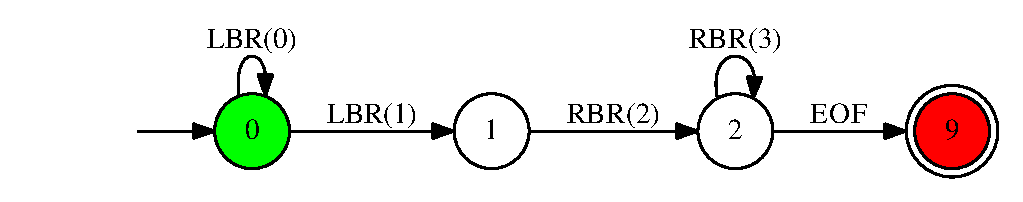
\includegraphics[scale=0.3]{dot/in3.eps}
   }  
   \hfill
    \subfloat[SPPF\label{resultSPPF}]{%
      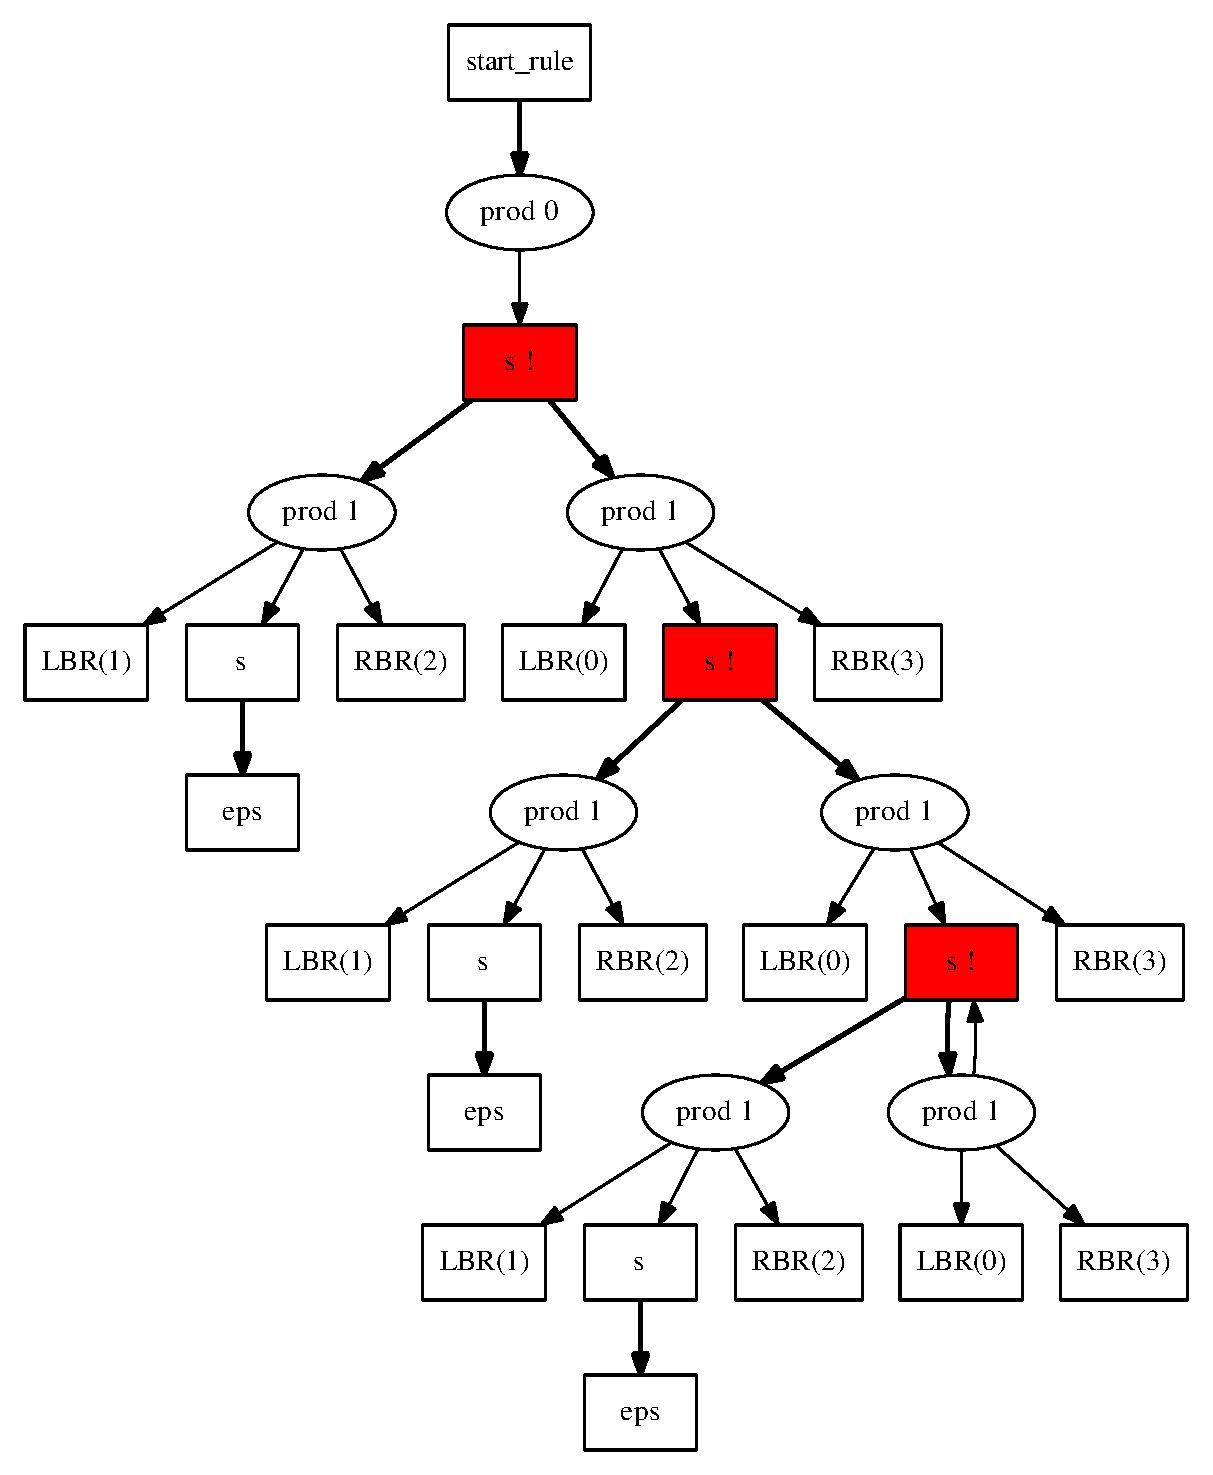
\includegraphics[scale=0.3]{dot/out3.eps}
    }
    \caption{Regular approximation and SPPF}
    \label{fig:SPPFforReg}
 \end{figure}

%\begin{figure}
%    \begin{center}
%        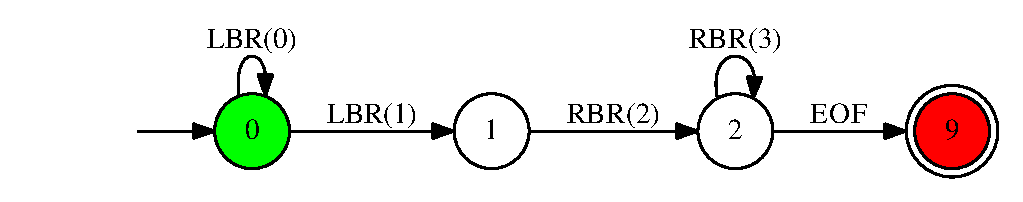
\includegraphics[scale=0.5]{dot/in3.eps}
%    \end{center}
%    \caption{$A_1$ -- input for our algorithm: regular approximation for string-embedded code after tokenization} 
%    \label{faApprox}
%\end{figure}

As it can be seen, some of the words from regular approximation do not belong to the reference language (for example, 
\verb|LBR LBR RBR|). The algorithm ignores such strings and constructs SPPF, which contains derivation trees 
for all recognized strings w.r.t. reference grammar.

%\begin{figure}
%    \begin{center}
%        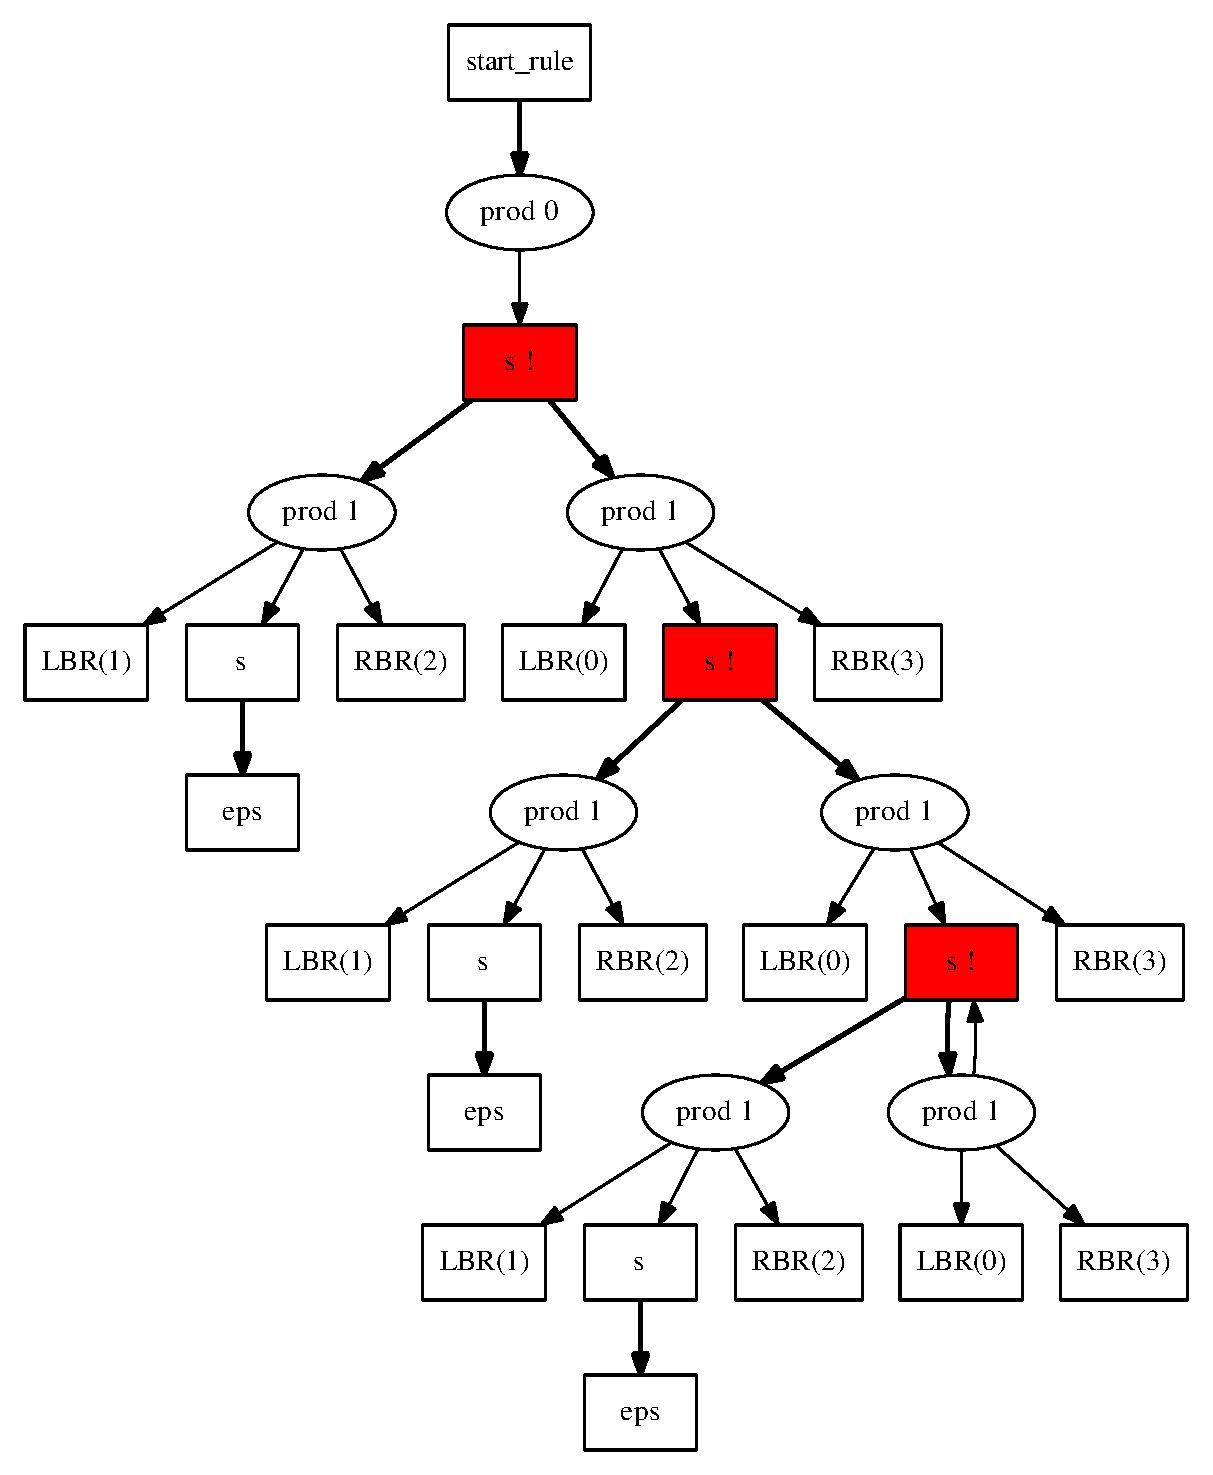
\includegraphics[scale=0.3]{dot/out3.eps}
%    \end{center}
%    \caption{SPPF for input FA presented in figure~\ref{faApprox}}
%    \label{resultSPPF}
%\end{figure}
\pagebreak
\section{\appendixname: RNGLR pseudocode}\label{RNGLRCode}

\begin{algorithm}[]
\begin{algorithmic}[1]
\caption{RNGLR algorithm}
\label{rnglr}
\Function{parse}{$grammar, input$}
  \State{$\mathcal{R} \gets \emptyset$} \Comment{Queue of tuples of GSS vertex, nonterminal, and reduction length}
  \State{$\mathcal{Q} \gets \emptyset$} \Comment{Collection of pairs of GSS vertex and parser state}
  \If{$input = \epsilon$}
    \If{$grammar$ accepts empty input} {report success}
    \Else { report failure}
    \EndIf
  \Else
    \State{\Call{addVertex}{$0, 0, startState$}}
    \ForAll{$i$ in $0..input.Length-1$}
      \State{\Call{reduce}{$i$}}
      \State{\Call{push}{$i$}}
    \EndFor
    \If{$i=input.Length-1$ and there is a vertex in the last level of GSS which state is accepting}
      \State{report success}
    \Else { report failure}
    \EndIf
  \EndIf
\EndFunction
\Function{reduce}{$i$}
  \While{$\mathcal{R}$ is not empty}
    \State{$(v, N, l) \gets \mathcal{R}.Dequeue()$}
    \State{find the set $\mathcal{X}$ of vertices reachable from $v$ along the path of length $(l-1)$}
    \State{or length $0$ if $l=0$}
    \ForAll{$v_{h} = (level_{h}, state_{h})$ in $\mathcal{X}$}
      \State{$state_{t} \gets$ calculate new state by $state_{h}$ and nonterminal $N$}
      \State{\Call{addEdge}{$i, v_{h}, v.level, state_{tail}, (l=0)$}}
    \EndFor
  \EndWhile
\EndFunction
\Function{push}{$i$}
  \State{$\mathcal{Q^{'}} \gets$ copy $\mathcal{Q}$}
  \While{$\mathcal{Q^{'}}$ is not empty}
    \State{$(v, state) \gets \mathcal{Q}.Dequeue()$}
    \State{\Call{addEdge}{$i, v, v.level + 1, state, false$}}
  \EndWhile
\EndFunction
\end{algorithmic}
\end{algorithm}

\begin{algorithm}[]
\begin{algorithmic}[1]
\caption{GSS construction}
\label{RNGLRMain}
\Function{addVertex}{$i, level, state$}
  \If{GSS does not contain vertex $v = (level, state)$}
    \State{add new vertex $v = (level, state)$ to GSS}
    \State{calculate the set of shifts by $v$ and the $input[i+1]$ and add them to $\mathcal{Q}$}
    \State{calculate the set of zero-reductions by $v$ and the $input[i+1]$ and}
    \State{add them to $\mathcal{R}$}
  \EndIf
  \State{\Return{$v$}}
\EndFunction
\Function{addEdge}{$i, v_{h}, level_{t}, state_{t}, isZeroReduction$}
  \State{$v_{t} \gets$ \Call{addVertex}{$i, level_{t}, state_{t}$}}
  \If{GSS does not contain edge from $v_{t}$ to $v_{h}$}
    \State{add new edge from $v_{t}$ to $v_{h}$ to GSS}
    \If{not $isZeroReduction$}
      \State{calculate the set of reductions by $v$ and the $input[i+1]$ and}
      \State{add them to $\mathcal{R}$}
    \EndIf
  \EndIf
\EndFunction
\end{algorithmic}
\end{algorithm}


        % Приложения

\end{document}
